%!TEX program = xelatex
\documentclass{article}
\usepackage[a4paper,left=2.5cm,right=2.5cm,top=2.2cm,bottom=2.2cm]{geometry}
\usepackage{listings}
\usepackage{float}
\usepackage{graphicx}
\graphicspath{{./}{Projects/One/Phase_2/}}
\usepackage{amsmath}
\usepackage{siunitx}
\usepackage{booktabs}
\usepackage{xcolor}
\usepackage{caption}
\usepackage[most]{tcolorbox}

\newtcolorbox{answerbox}{
    enhanced,
    breakable,
    colback=blue!6,
    colframe=blue!6,
    boxrule=0pt,
    arc=2pt,
    left=6pt,
    right=6pt,
    top=6pt,
    bottom=6pt,
    fontupper=\small
}

\sisetup{per-mode=reciprocal, inter-unit-product = \cdot}

\title{\textbf{Spring'\ 26 \; Introduction to Biological Intelligence: Brain Simulation\\ \textcolor{red}{Project 1 Part 2 \& 3 :} Experiment \& Analysis}}
\author{}
\date{}

\begin{document}
\pagestyle{plain}
\maketitle

\vspace{-3.5em}

\begin{center}
\Large
\textbf{Yian Li (PKU, 2300017854)}\\
\textbf{ZiHang Xu (THU, 2023010082)}\\
\textbf{WeiJun Hong (PKU, 2400017452)}
\end{center}
\vspace{0.5em}

\clearpage

\section*{\textbf{Q1.} Implement an Active Point Neuron Model in NEURON}

\textbf{Experiment.}
Construct a point neuron model in \textsc{NEURON} consisting of a single section with one segment, and insert the \texttt{hh1} channel mechanism.
Apply a constant current injection to trigger an action potential.

Simulate the model and plot the time courses of:
\begin{itemize}
    \item the membrane potential $V_m$;
    \item ionic currents: $I_{\scriptscriptstyle\text{Na}}$ and $I_{\scriptscriptstyle\text{K}}$;
    \item gating variables: $m,\,h$ (for $\textrm{Na}^+$) and $n$ (for $\textrm{K}^+$);
    \item conductances: $g_{\scriptscriptstyle\text{Na}}$ and $g_{\scriptscriptstyle\text{K}}$.
\end{itemize}

\noindent\textbf{Parameter set} (using the default units in \textsc{NEURON}):

\begin{itemize}
    \item $\texttt{L} = \SI{10}{\micro\meter}$;
    \item $\texttt{diam} = \SI{10}{\micro\meter}$;
    \item $\texttt{Ra} = \SI{100}{\ohm\centi\meter}$;
    \item $\texttt{cm} = \SI{1}{\micro\farad\per\centi\meter\squared}$;
    \item $\texttt{hh1.gnabar} = \SI{0.12}{\siemens\per\centi\meter\squared}$;
    \item $\texttt{hh1.gkbar} = \SI{0.036}{\siemens\per\centi\meter\squared}$;
    \item $\texttt{hh1.gl} = \SI{0.0003}{\siemens\per\centi\meter\squared}$;
    \item injected current amplitude: $\SI{0.05}{\nano\ampere}$;
    \item injected current duration: $\SI{0.5}{\milli\second}$.
\end{itemize}

\noindent\textbf{Report requirements.}
In your report, \textit{include all plots} and \textit{briefly interpret} them.
\emph{Explain} how the gating variables shape the different phases of an action potential:

\begin{enumerate}
    \item \textbf{Rising phase (depolarization):} the membrane potential rapidly becomes more positive.
    \item \textbf{Peak phase:} the membrane potential reaches its maximum value.
    \item \textbf{Falling phase (repolarization):} the membrane potential returns toward the resting level.
    \item \textbf{Afterhyperpolarization:} the membrane potential temporarily becomes more negative than the resting potential.
    \item \textbf{Refractory period:} during which initiating another action potential is impossible or difficult.
\end{enumerate}

\textbf{Hint question:} Plot the voltage-dependency of the time constants $\tau_x$ and steady-state values $x_{\infty}$ of the gating variables.
You may discover that the steady-state sodium current $\bar{g}_{\scriptscriptstyle\text{Na}}m_{\infty}^3h_{\infty}(V_m-E_{\scriptscriptstyle\text{Na}})$ (also known as the \textit{window current}) is always very small.
Then, how is the large sodium current obtained?

\begin{answerbox}
\textbf{Results.} The simulation output is shown in Figure~\ref{fig:q1_main}.
\begin{center}
    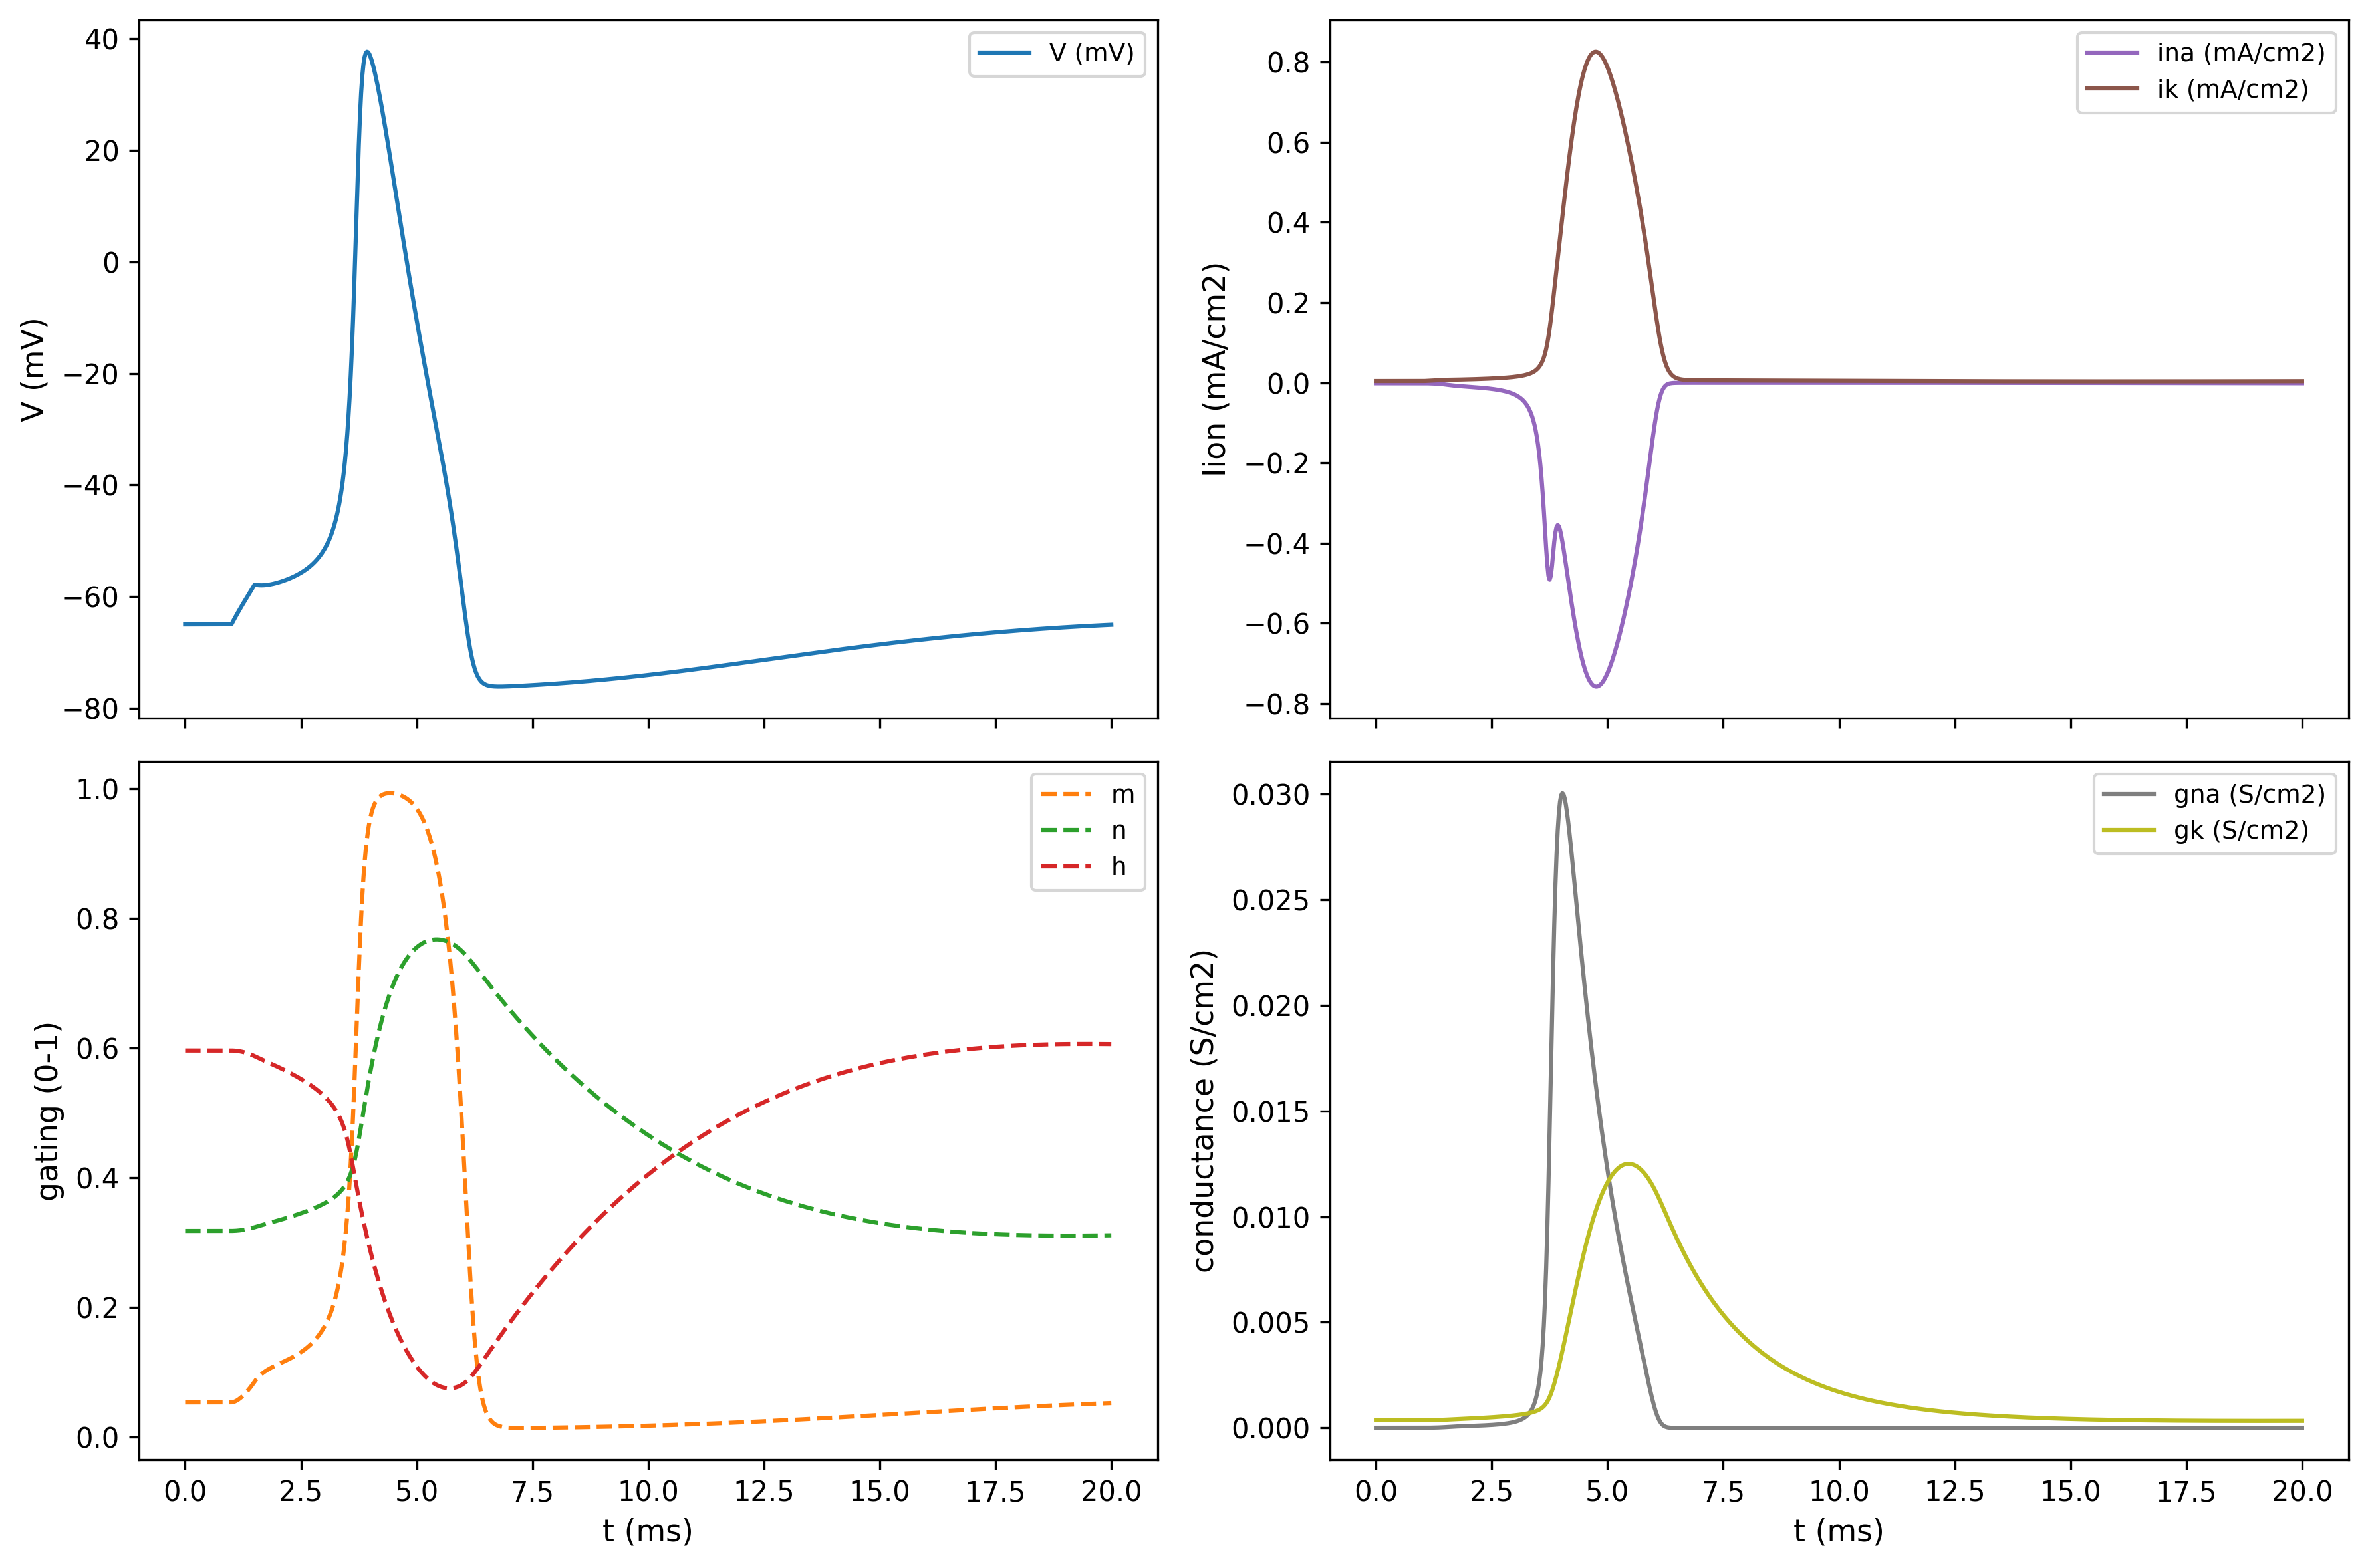
\includegraphics[width=0.98\linewidth]{Project_Code/Question_1/simulator.png}
    \captionof{figure}{Q1 results. Top-left: membrane voltage $V_m(t)$. Top-right: ionic currents $I_{\mathrm{Na}}(t)$ and $I_{\mathrm{K}}(t)$. Bottom-left: gating variables $m,h,n$. Bottom-right: conductances $g_{\mathrm{Na}}(t)$ and $g_{\mathrm{K}}(t)$.}
    \label{fig:q1_main}
\end{center}

\textbf{Interpretation (gating variables and AP phases).}
\begin{itemize}
    \item \textbf{Rising phase:} depolarization rapidly increases $m$ (fast activation, small $\tau_m$), which increases $g_{\mathrm{Na}}=\bar g_{\mathrm{Na}}m^3h$ and produces a large inward $I_{\mathrm{Na}}$ (positive feedback).
    \item \textbf{Peak:} $h$ decreases (Na inactivation) while $n$ increases (K activation). The inward Na current weakens and the outward K current strengthens.
    \item \textbf{Falling phase:} delayed but sustained $n$ keeps $g_{\mathrm{K}}=\bar g_{\mathrm{K}}n^4$ high, driving repolarization.
    \item \textbf{Afterhyperpolarization:} $n$ decays slowly, so $g_K$ remains elevated briefly, pushing $V_m$ below rest.
    \item \textbf{Refractory period:} shortly after a spike, $h$ is still low (Na channels unavailable) and $n$ still high (strong outward current), making re-initiation difficult.
\end{itemize}

\textbf{Window current hint.} The steady-state ``window'' factor $m_\infty^3h_\infty$ is small near rest, so the steady-state Na current is small. During a spike, however, $m$ responds much faster than $h$ and $n$: transiently, $m$ can become large while $h$ has not fully inactivated yet and $n$ has not fully activated, creating a short time window with large $g_{\mathrm{Na}}$ and thus a large inward $I_{\mathrm{Na}}$.
\end{answerbox}

\clearpage

\section*{\textbf{Q2.} Explore the Conditions for Spike Initiation}

In \textbf{Q1}, you used the following stimulus to evoke an action potential:
\begin{itemize}
    \item injected current amplitude: $I = \SI{0.05}{\nano\ampere}$;
    \item injected current duration: $\SI{0.5}{\milli\second}$.
\end{itemize}

\noindent\textbf{Experiment.}
Now vary the \emph{amplitude} and/or \emph{duration} of the injected current to explore the conditions under which the point neuron generates an action potential.

Compare cases in which the neuron \emph{does} spike with cases in which it \emph{does not}.
What differences do you observe in the voltage trajectories? Submit as least one plot for each case.\\

\noindent\textbf{Report requirements.}
In your report, explore the following question:

What are the exact conditions under which a spike is initiated?
Does the membrane potential have to exceed a particular threshold value $V_{\text{th}}$?
Or is there a minimal injected current $I_{\text{th}}$?
Or does spike initiation require that a certain amount of electrical charge $Q_{\text{th}}$ be delivered to the membrane?

You are not expected to give a perfectly rigorous answer. Instead, use your calculations together with the following approximation to develop an intuitive explanation of why one often speaks of a \textit{voltage threshold}.

\textbf{Hint.}
Consider the relation between ionic current and membrane potential, i.e.\ the $I_{\mathrm{ion}}$--$V_m$ relation.

Because the time constant of $m$ is roughly an order of magnitude smaller than those of $n$ and $h$ over a wide voltage range, a brief stimulus with duration comparable to $\tau_m$ may be analyzed using the approximation that $n$ and $h$ remain near their resting values, while $m$ adjusts instantaneously to its steady-state value at the new voltage:

\[
I_{\mathrm{ion}}(V_m)\approx
\bar g_{\scriptscriptstyle\mathrm{Na}}\,m_\infty(V_m)^3\,h(V_{\mathrm{rest}})\,(V_m-E_{\scriptscriptstyle\mathrm{Na}})
+
\bar g_{\scriptscriptstyle\mathrm{K}}\,n(V_{\mathrm{rest}})^4\,(V_m-E_{\scriptscriptstyle\mathrm{K}})
+
g_l\,(V_m-E_l).
\]

\textbf{Remark.}
Since this argument relies on an approximation, the threshold predicted by this analysis will not be exact. The goal here is to build physical intuition rather than to derive a numerically precise threshold.

\begin{answerbox}
\textbf{Representative cases.} We compare one non-spiking and one spiking stimulus (same duration, different amplitude).

\begin{center}
\begin{minipage}{0.49\linewidth}
    \centering
    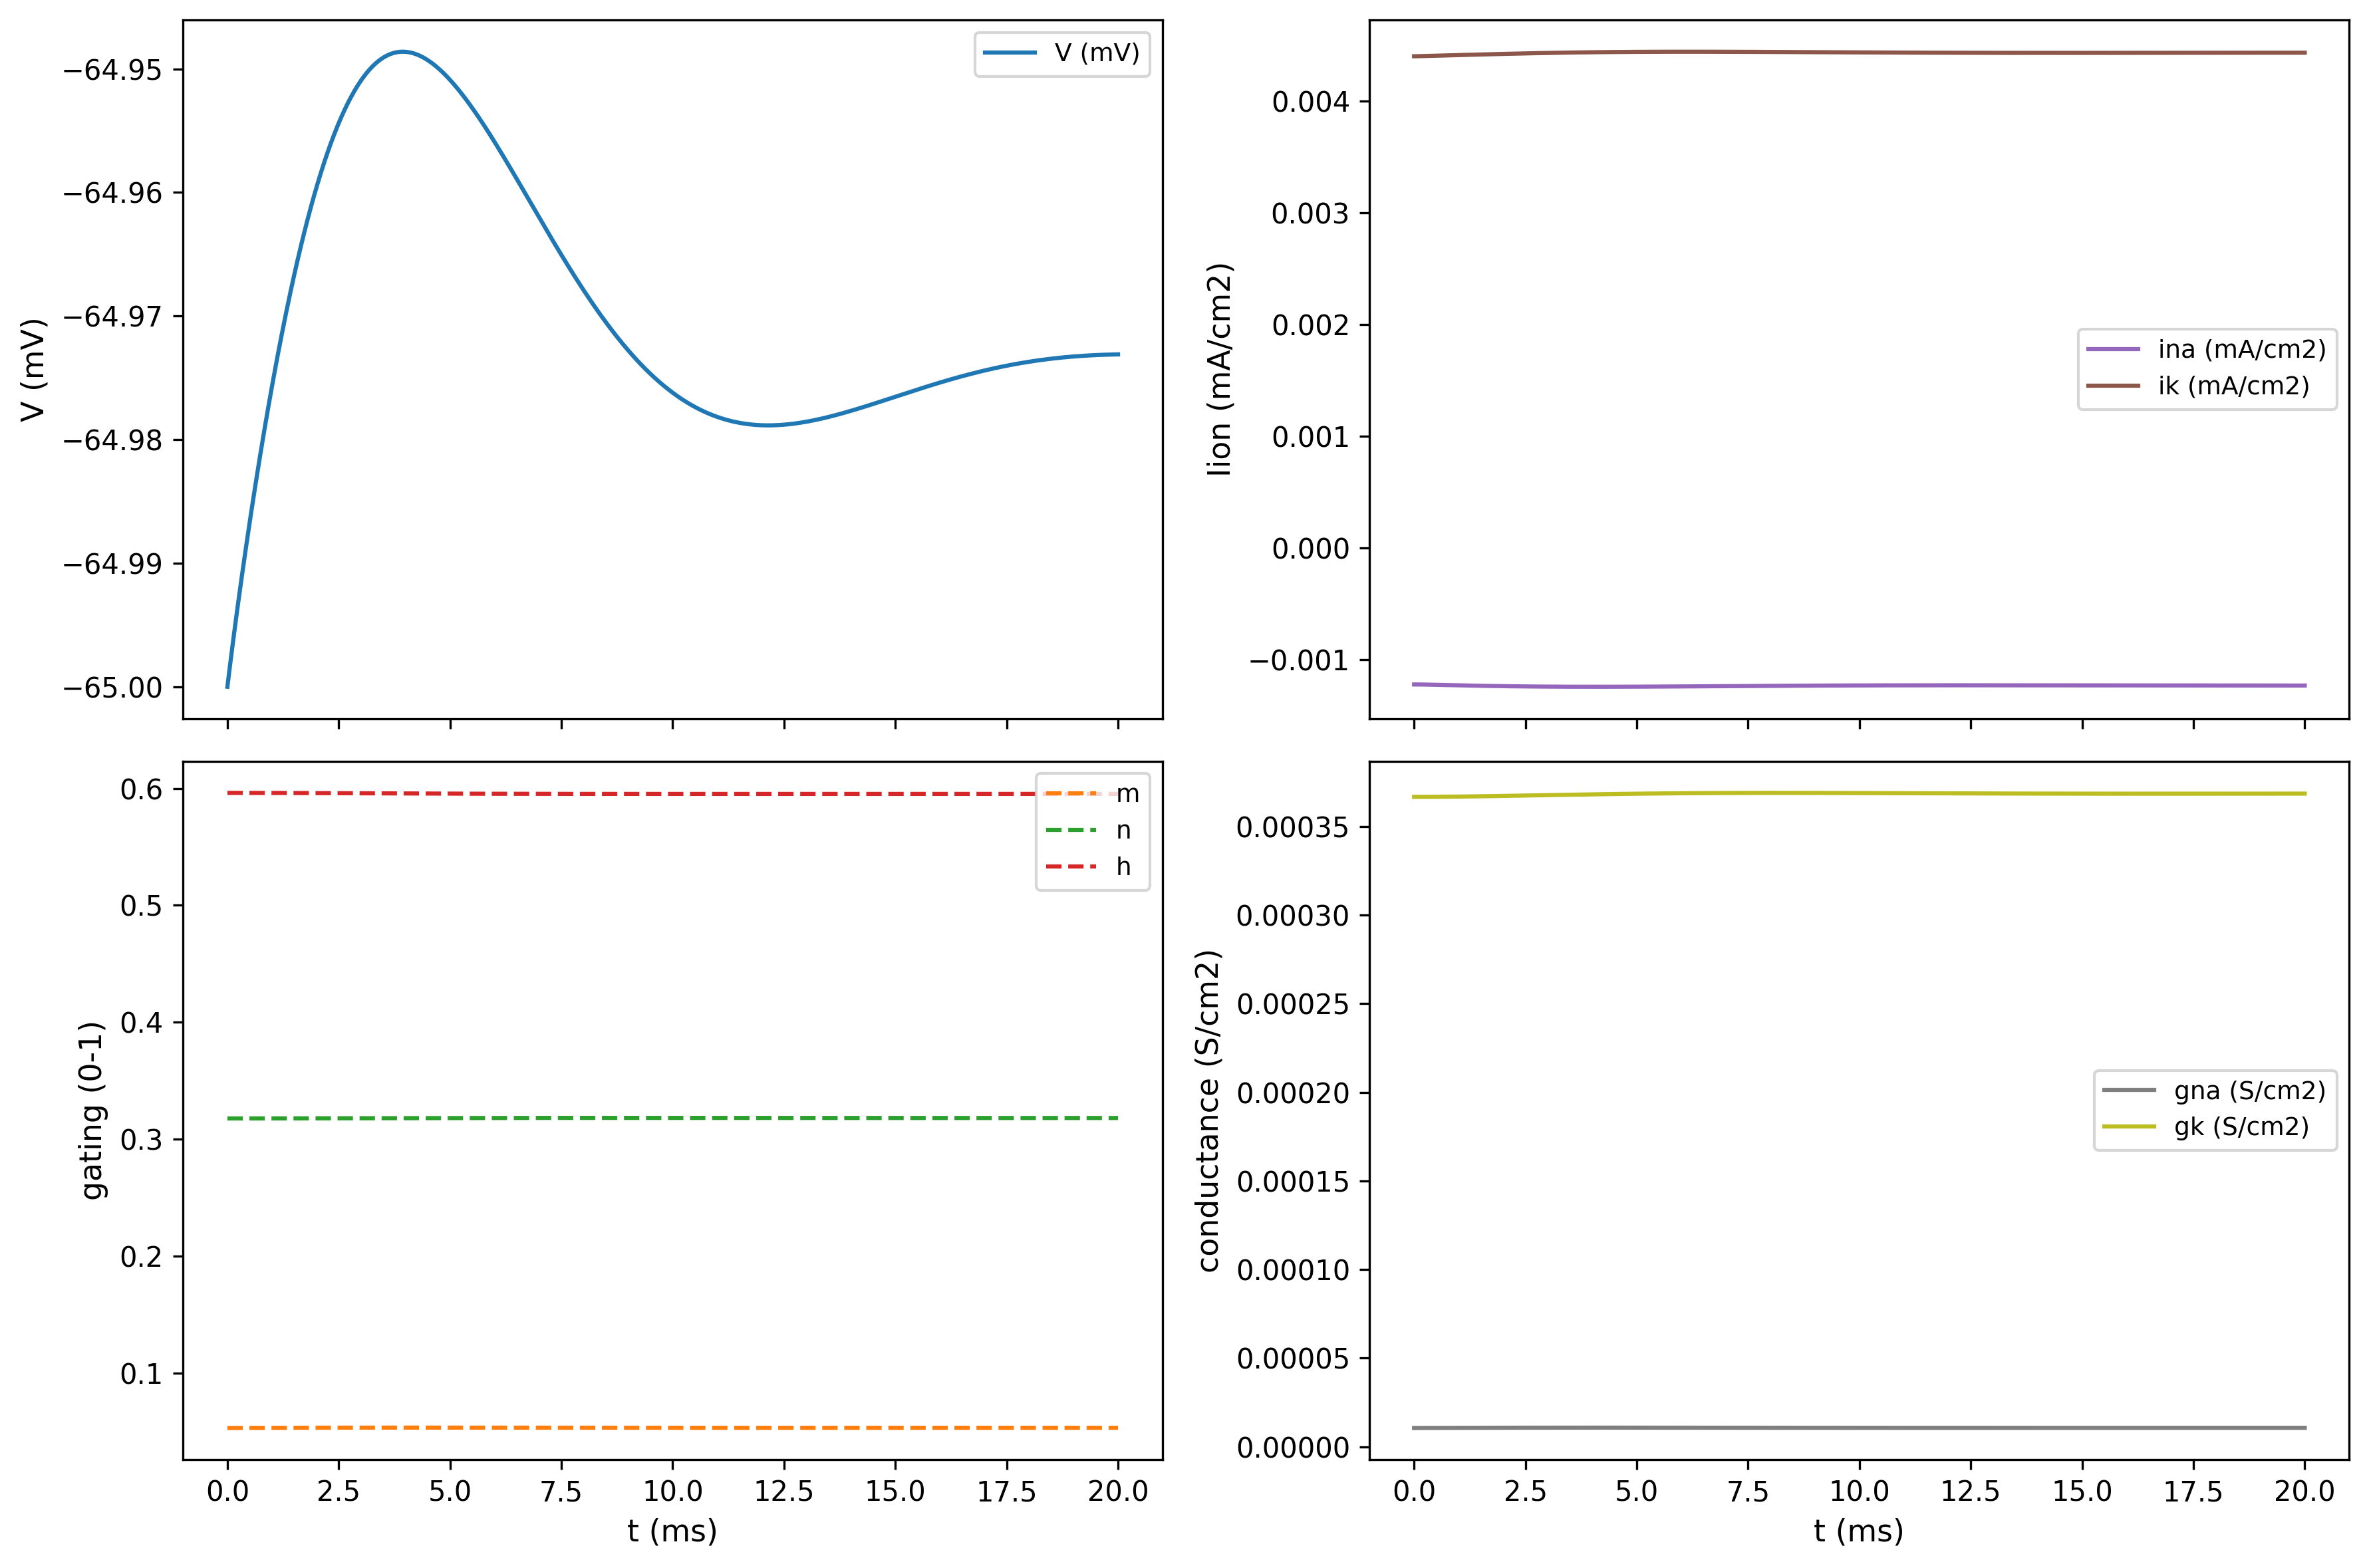
\includegraphics[width=\linewidth]{Project_Code/Question_2/fig/V_I_g_cond__amp_0nA__dur_0.5ms.png}
    \captionof{figure}{No spike: $I=0\,$nA, $\mathrm{dur}=0.5\,$ms. The voltage shows only a tiny passive deflection; gating variables remain near rest.}
\end{minipage}\hfill
\begin{minipage}{0.49\linewidth}
    \centering
    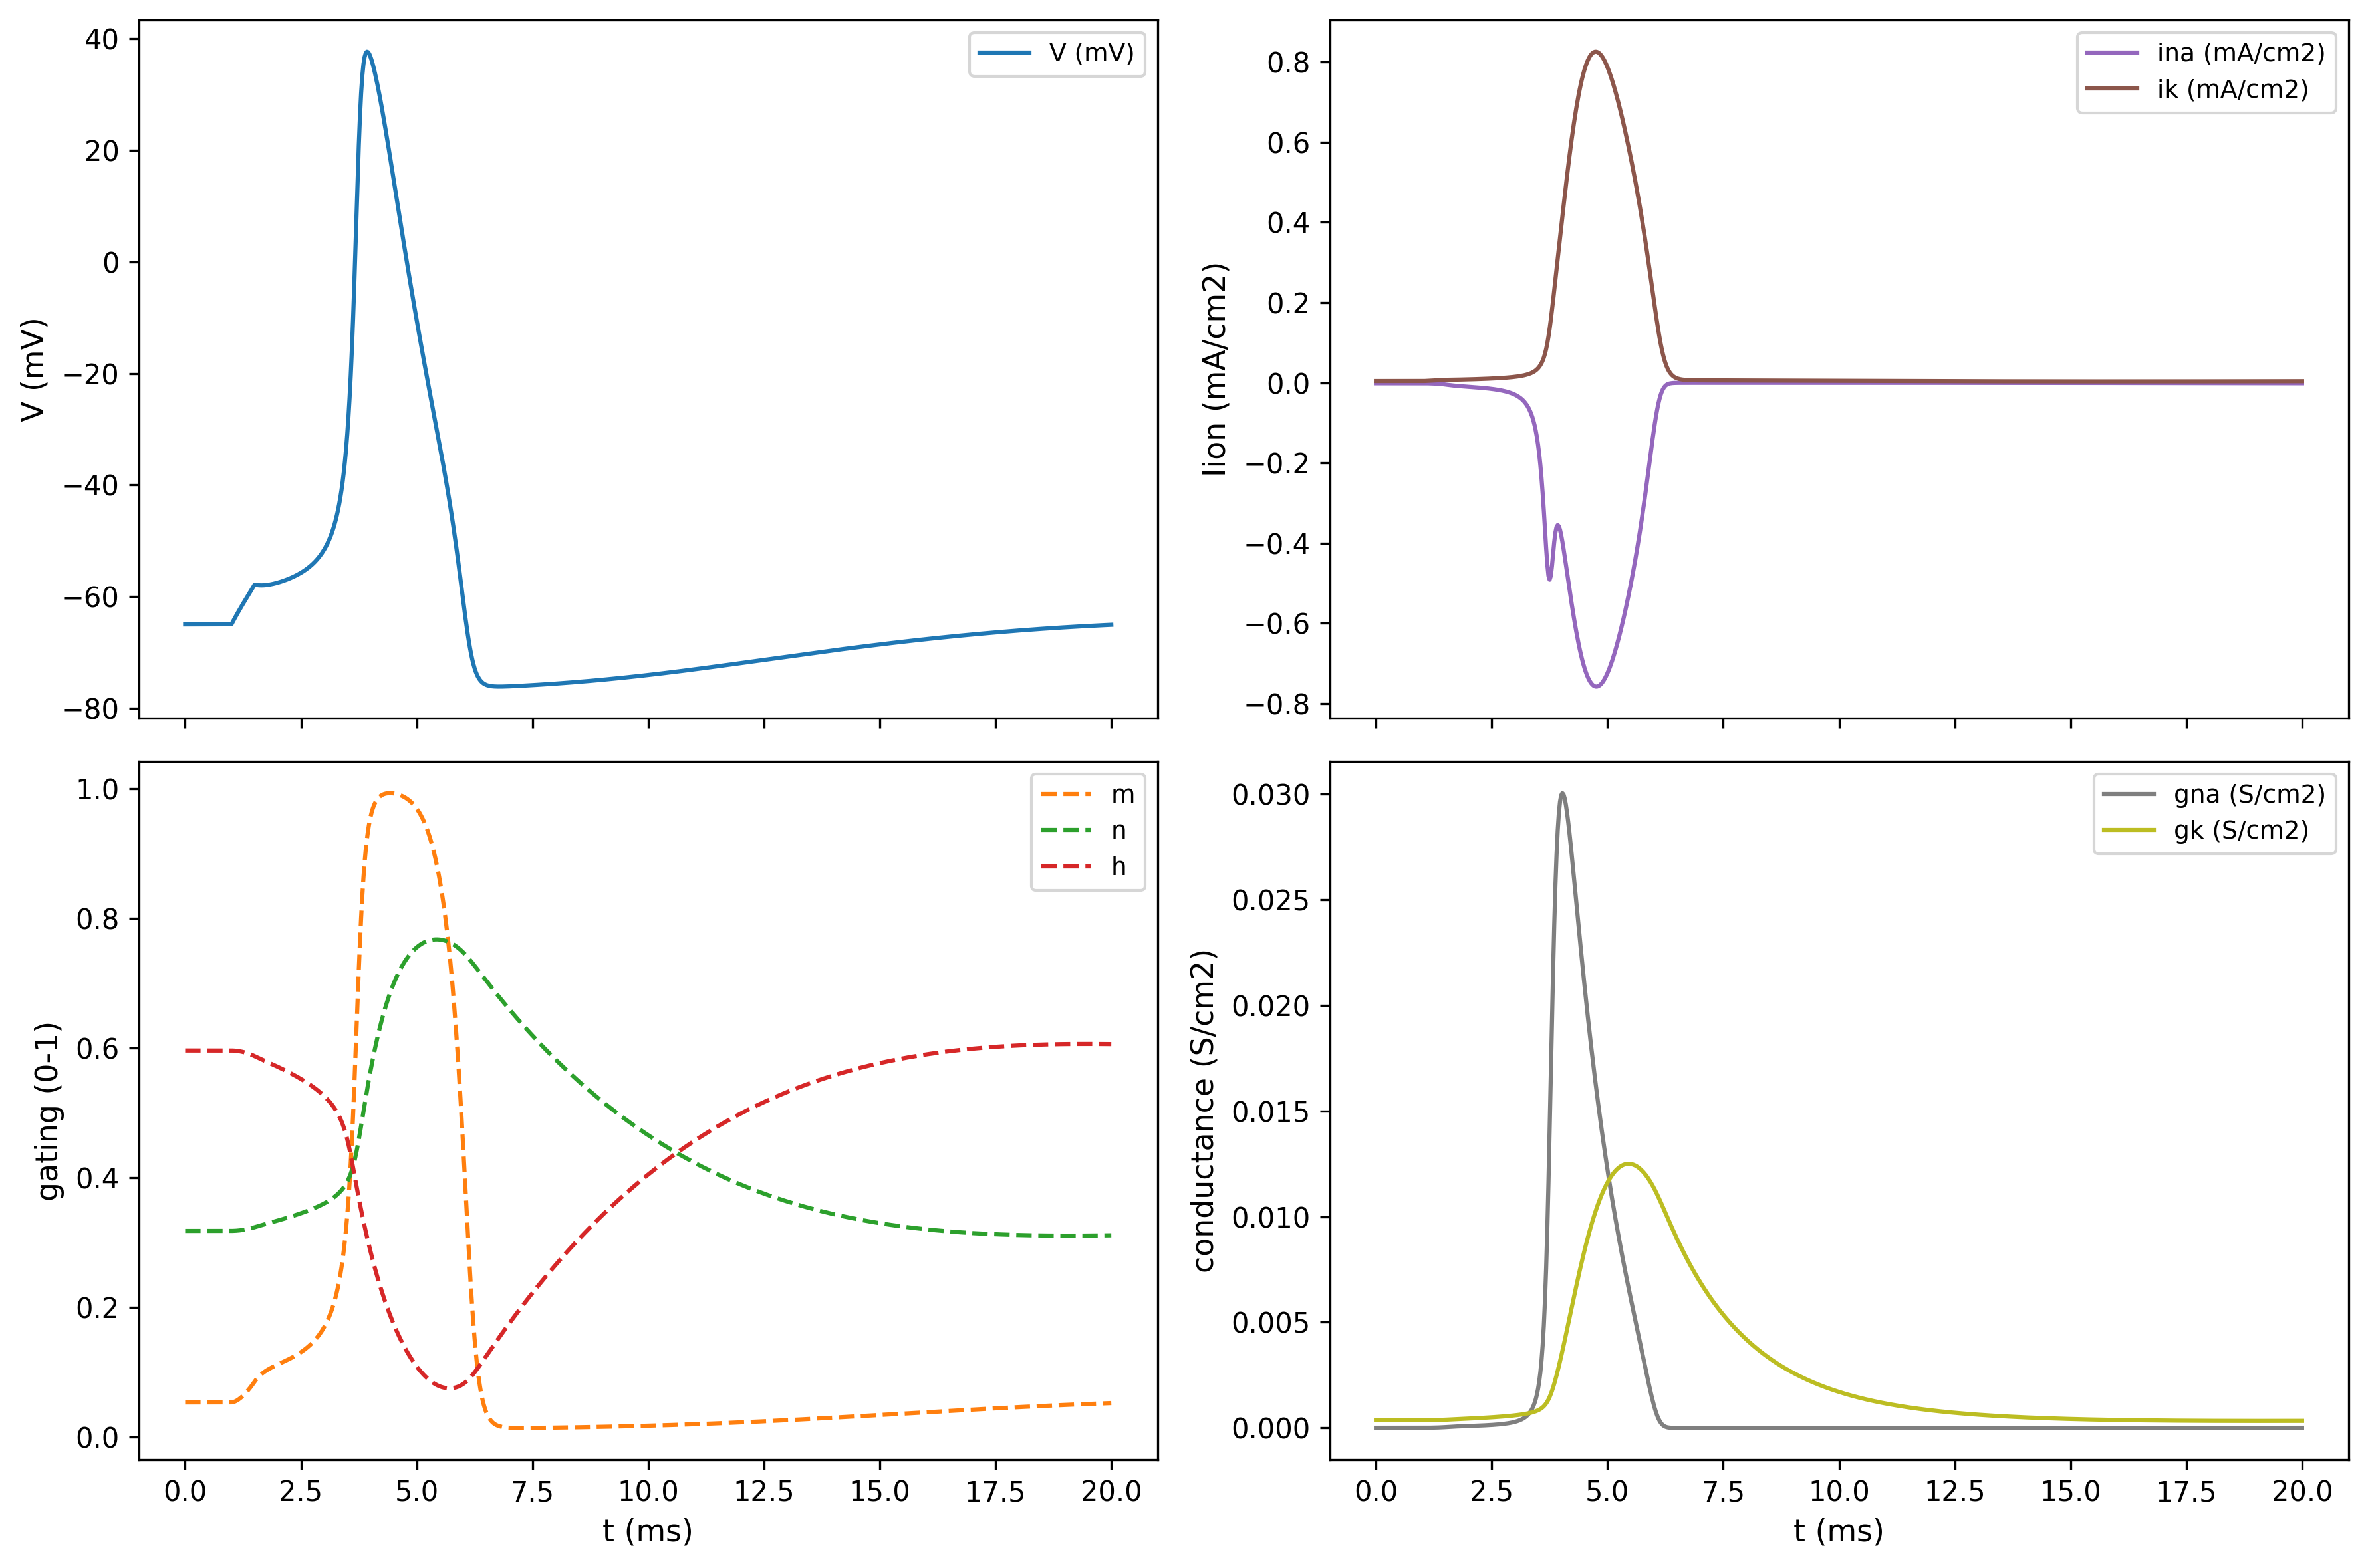
\includegraphics[width=\linewidth]{Project_Code/Question_2/fig/V_I_g_cond__amp_0.05nA__dur_0.5ms.png}
    \captionof{figure}{Spike: $I=0.05\,$nA, $\mathrm{dur}=0.5\,$ms. A regenerative upstroke occurs as $m$ increases rapidly, producing a large inward $I_{\mathrm{Na}}$.}
\end{minipage}
\end{center}

\textbf{Boundary in the $I$--duration plane.} To summarize the condition for spike initiation across many stimuli, we compute whether each $(I,\mathrm{dur})$ pair produces at least one spike, and extract the \emph{minimal} current amplitude that spikes for each duration (a strength--duration threshold curve). This produces an empirical phase boundary: points above the curve spike; points below do not.

\begin{center}
\begin{minipage}{0.49\linewidth}
    \centering
    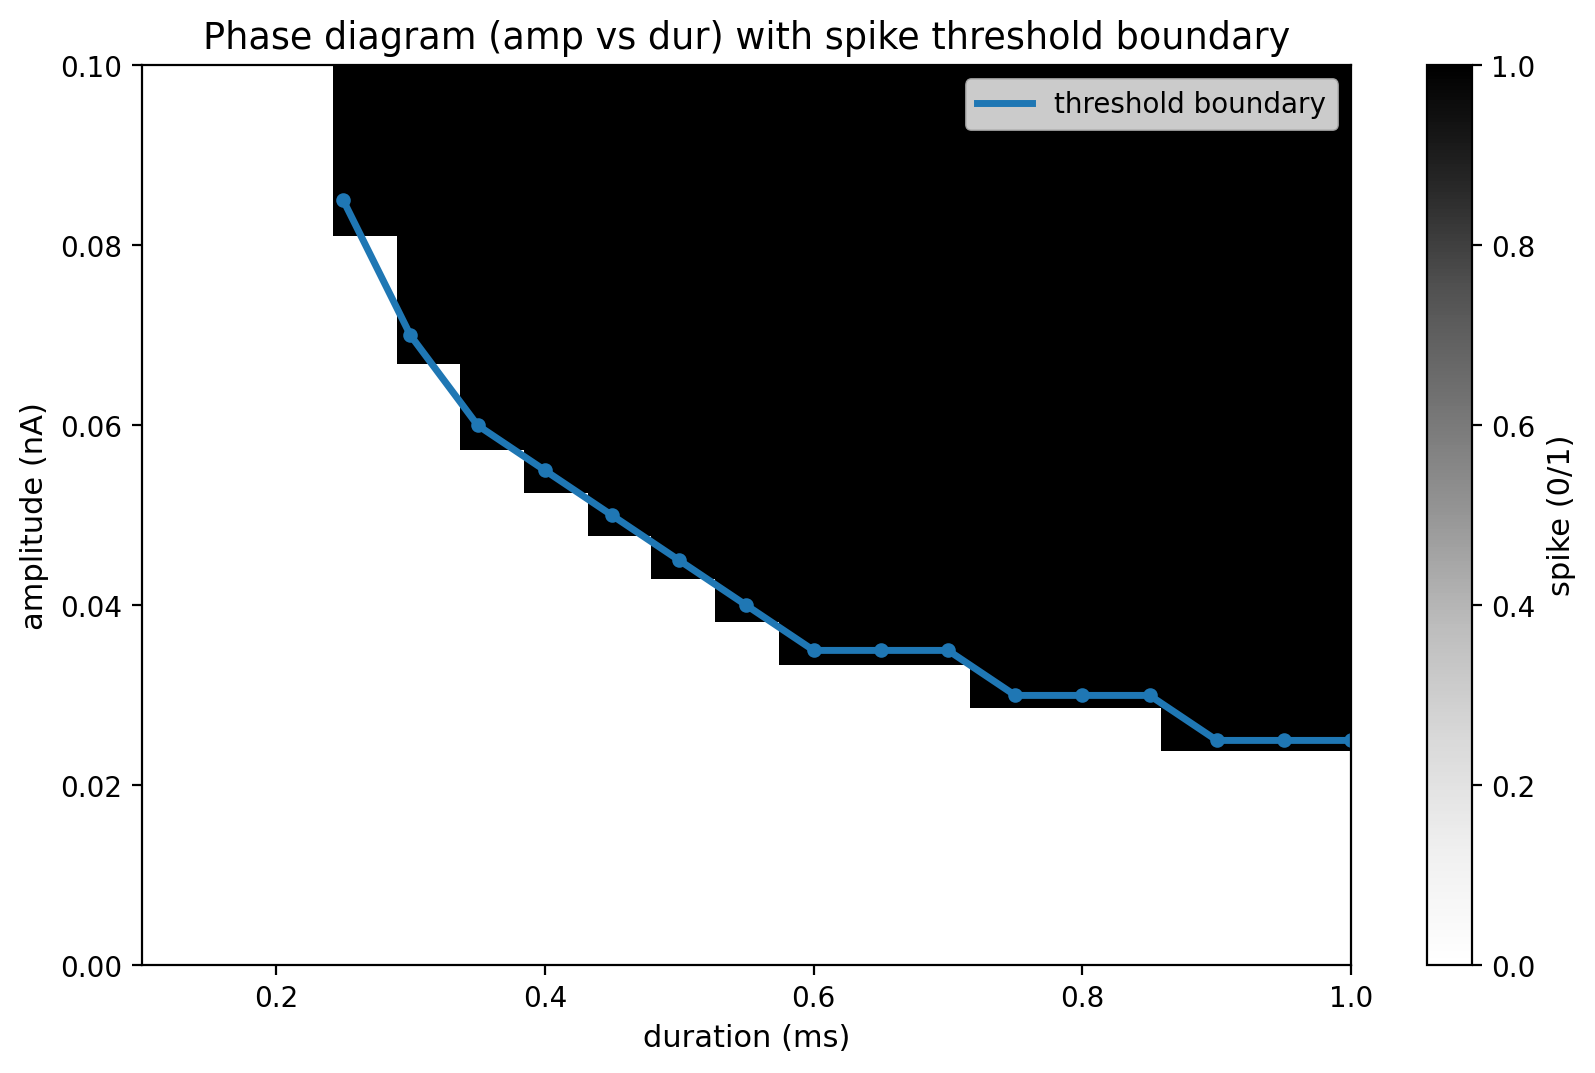
\includegraphics[width=\linewidth]{Project_Code/Question_2/phase_boundary_amp_dur.png}
    \captionof{figure}{Phase diagram in $(I,\mathrm{dur})$ with the extracted spike-threshold boundary (first-spike criterion). The boundary shifts upward for shorter durations, reflecting that brief pulses require larger amplitude to depolarize the membrane into the regenerative regime.}
\end{minipage}\hfill
\begin{minipage}{0.49\linewidth}
    \centering
    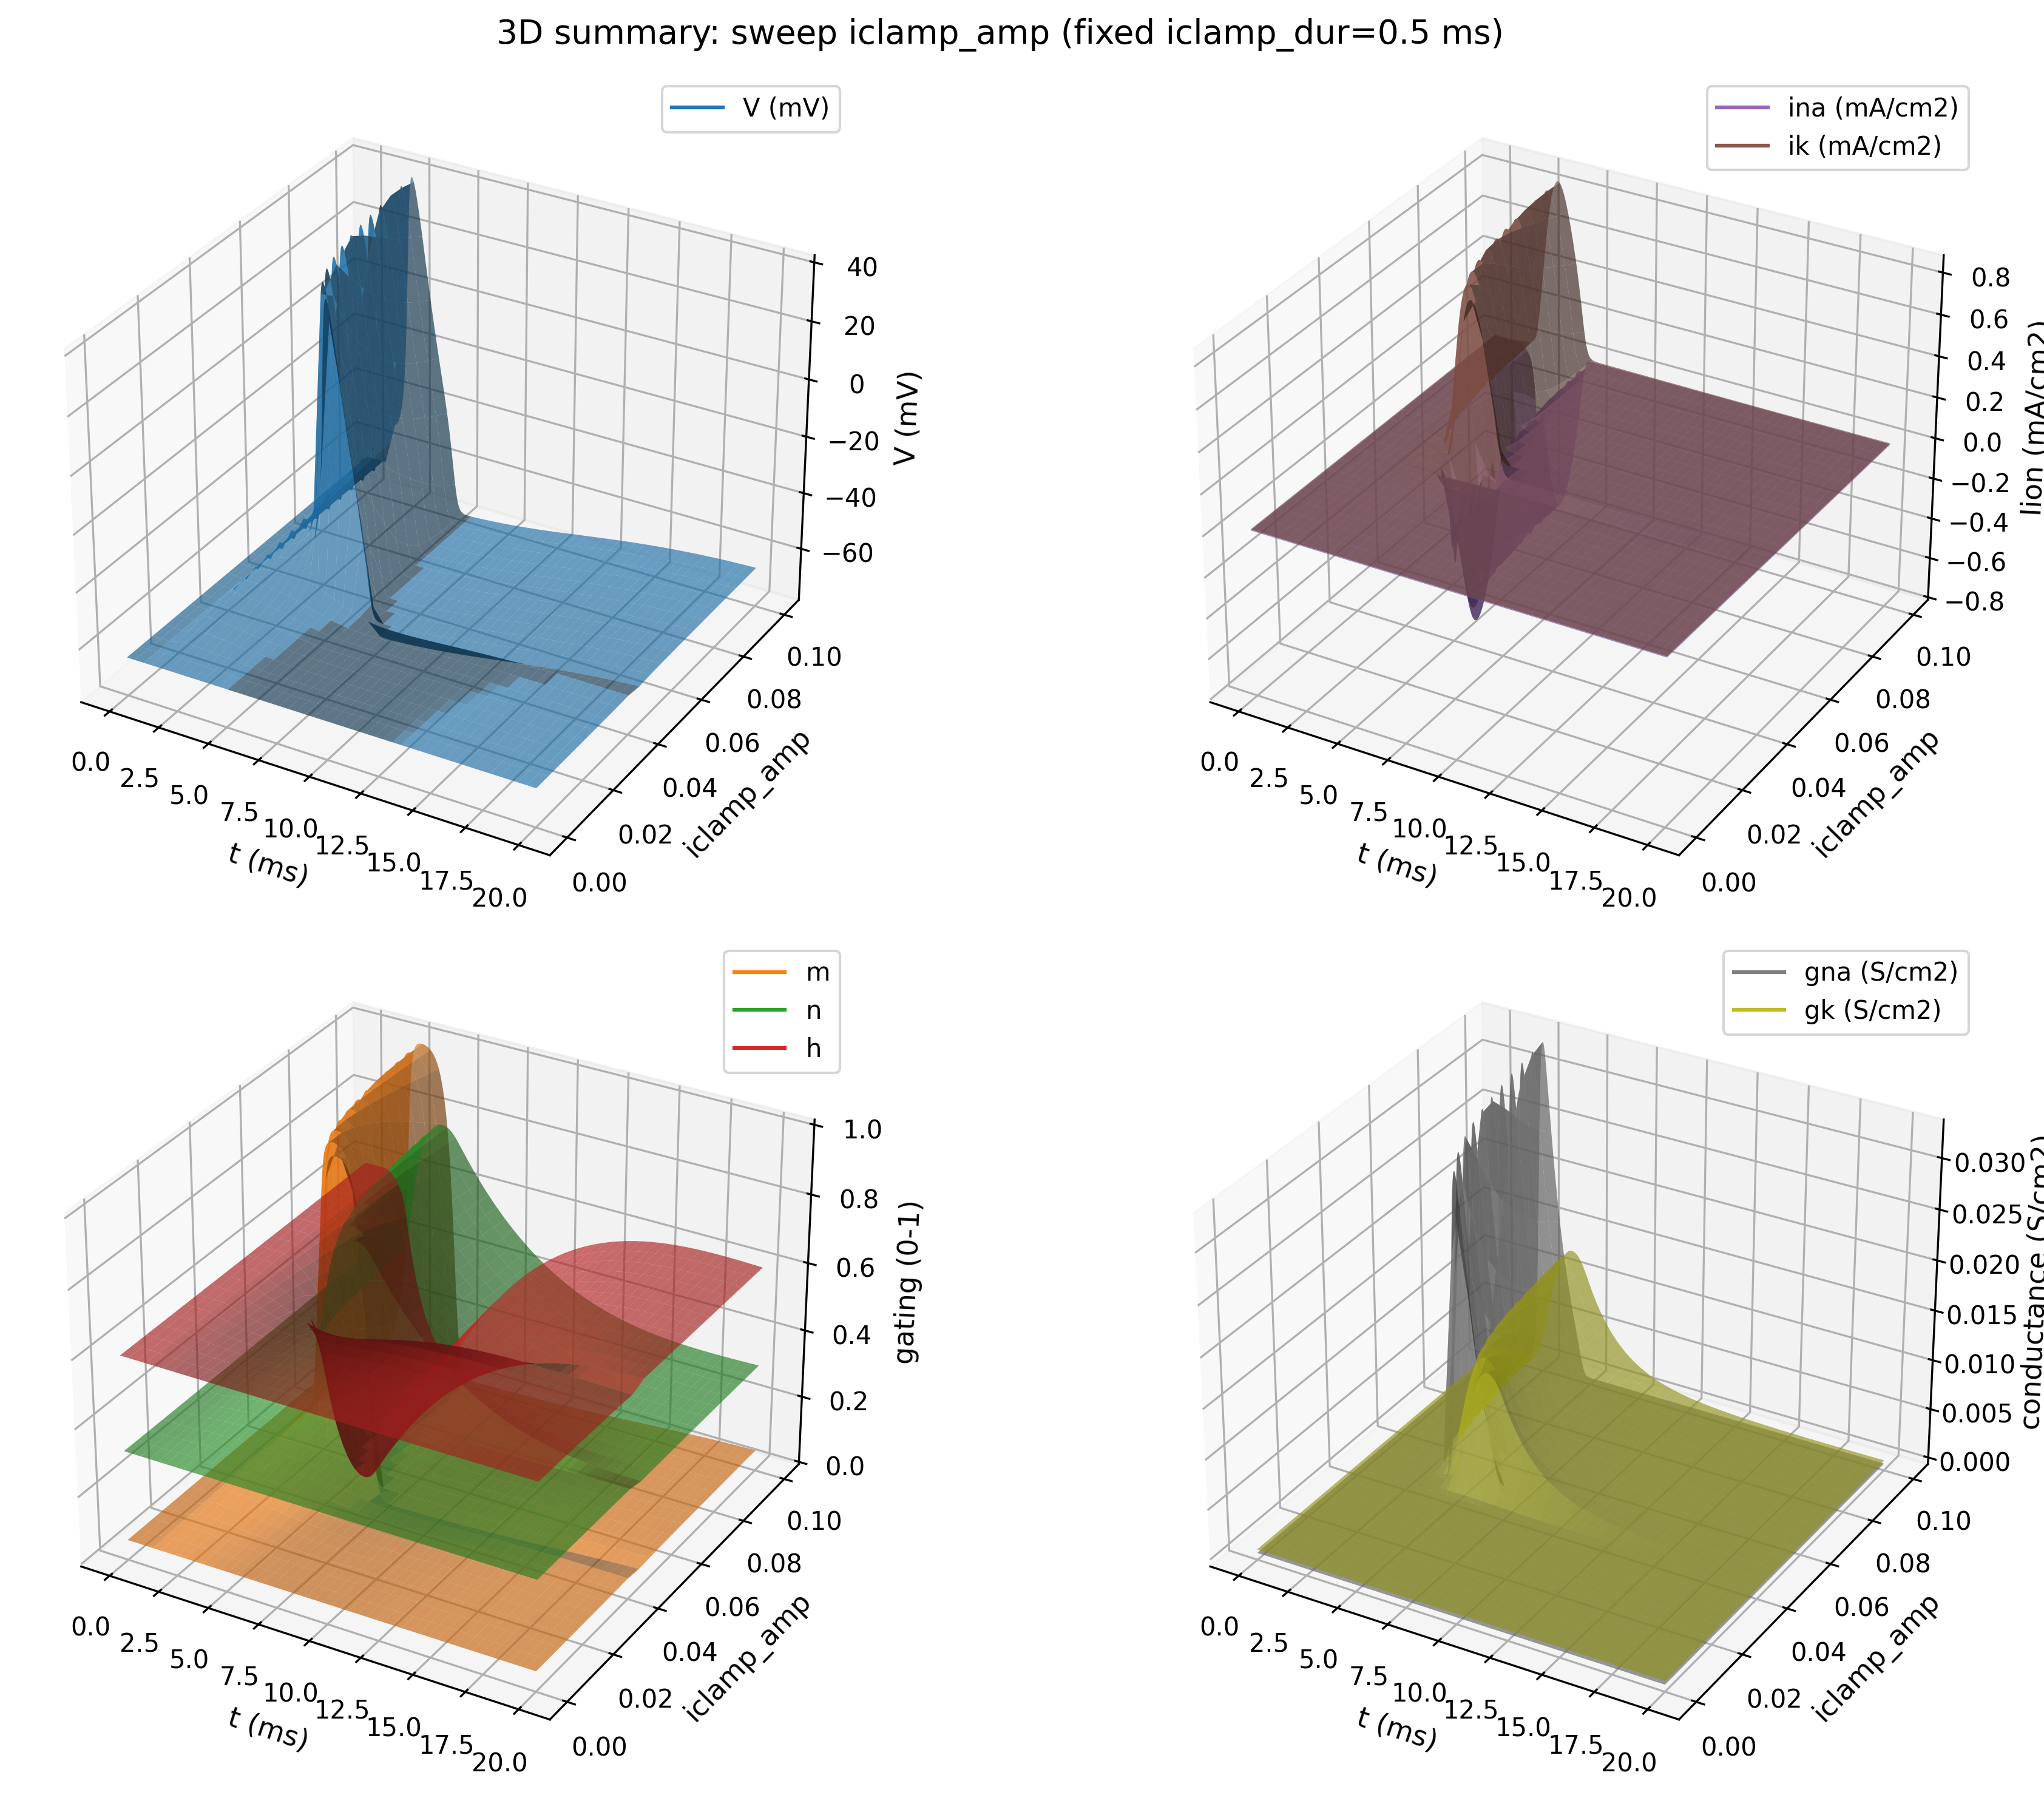
\includegraphics[width=\linewidth]{Project_Code/Question_2/summary_3d_sweep_amp.png}
    \captionof{figure}{3D visualization (example): sweeping stimulus amplitude at fixed duration shows how $V_m$, ionic currents, gating variables, and conductances transition from subthreshold responses to a full action potential as $I$ increases.}
\end{minipage}
\end{center}

\textbf{What is the ``exact'' spike-initiation condition?} In general, it is not a single fixed number (not a universal $V_{\mathrm{th}}$, $I_{\mathrm{th}}$, or $Q_{\mathrm{th}}$) because spike initiation is a dynamical, state-dependent process. However, for brief stimuli where $m$ is fast and $n,h$ remain near their resting values, the ionic current can be approximated as a nonlinear function $I_{\mathrm{ion}}(V_m)$.
In that approximation, the balance between injected current and ionic current can create an \emph{unstable} equilibrium (a ``threshold'') in the $I$--$V$ relation: once $V_m$ is pushed beyond this point, the rapid increase of $m_\infty(V_m)$ makes $I_{\mathrm{Na}}$ dominate and drives a runaway depolarization (spike). This provides the usual intuition for why one often speaks of a \emph{voltage threshold}.

\textbf{$I$--$V$ curve with stable/unstable equilibria.} A convenient way to visualize the ``threshold'' is to plot the approximate ionic $I$--$V$ relation $I_{\mathrm{ion}}(V)$ (using the hint approximation: freeze $h,n$ near rest and let $m$ relax quickly). For a fixed injected current density $I_{\mathrm{inj}}$, equilibria satisfy
\[
I_{\mathrm{inj}} = I_{\mathrm{ion}}(V^*).
\]
Linear stability follows from the reduced 1D balance $C\,\mathrm{d}V/\mathrm{d}t = I_{\mathrm{inj}} - I_{\mathrm{ion}}(V)$: an equilibrium is \emph{stable} if $\left.\mathrm{d}I_{\mathrm{ion}}/\mathrm{d}V\right|_{V^*} > 0$ (green dot), and \emph{unstable} if the slope is negative (red cross). The unstable fixed point serves as a separatrix: voltages pushed beyond it tend to enter the regenerative (spiking) regime.

\begin{center}
    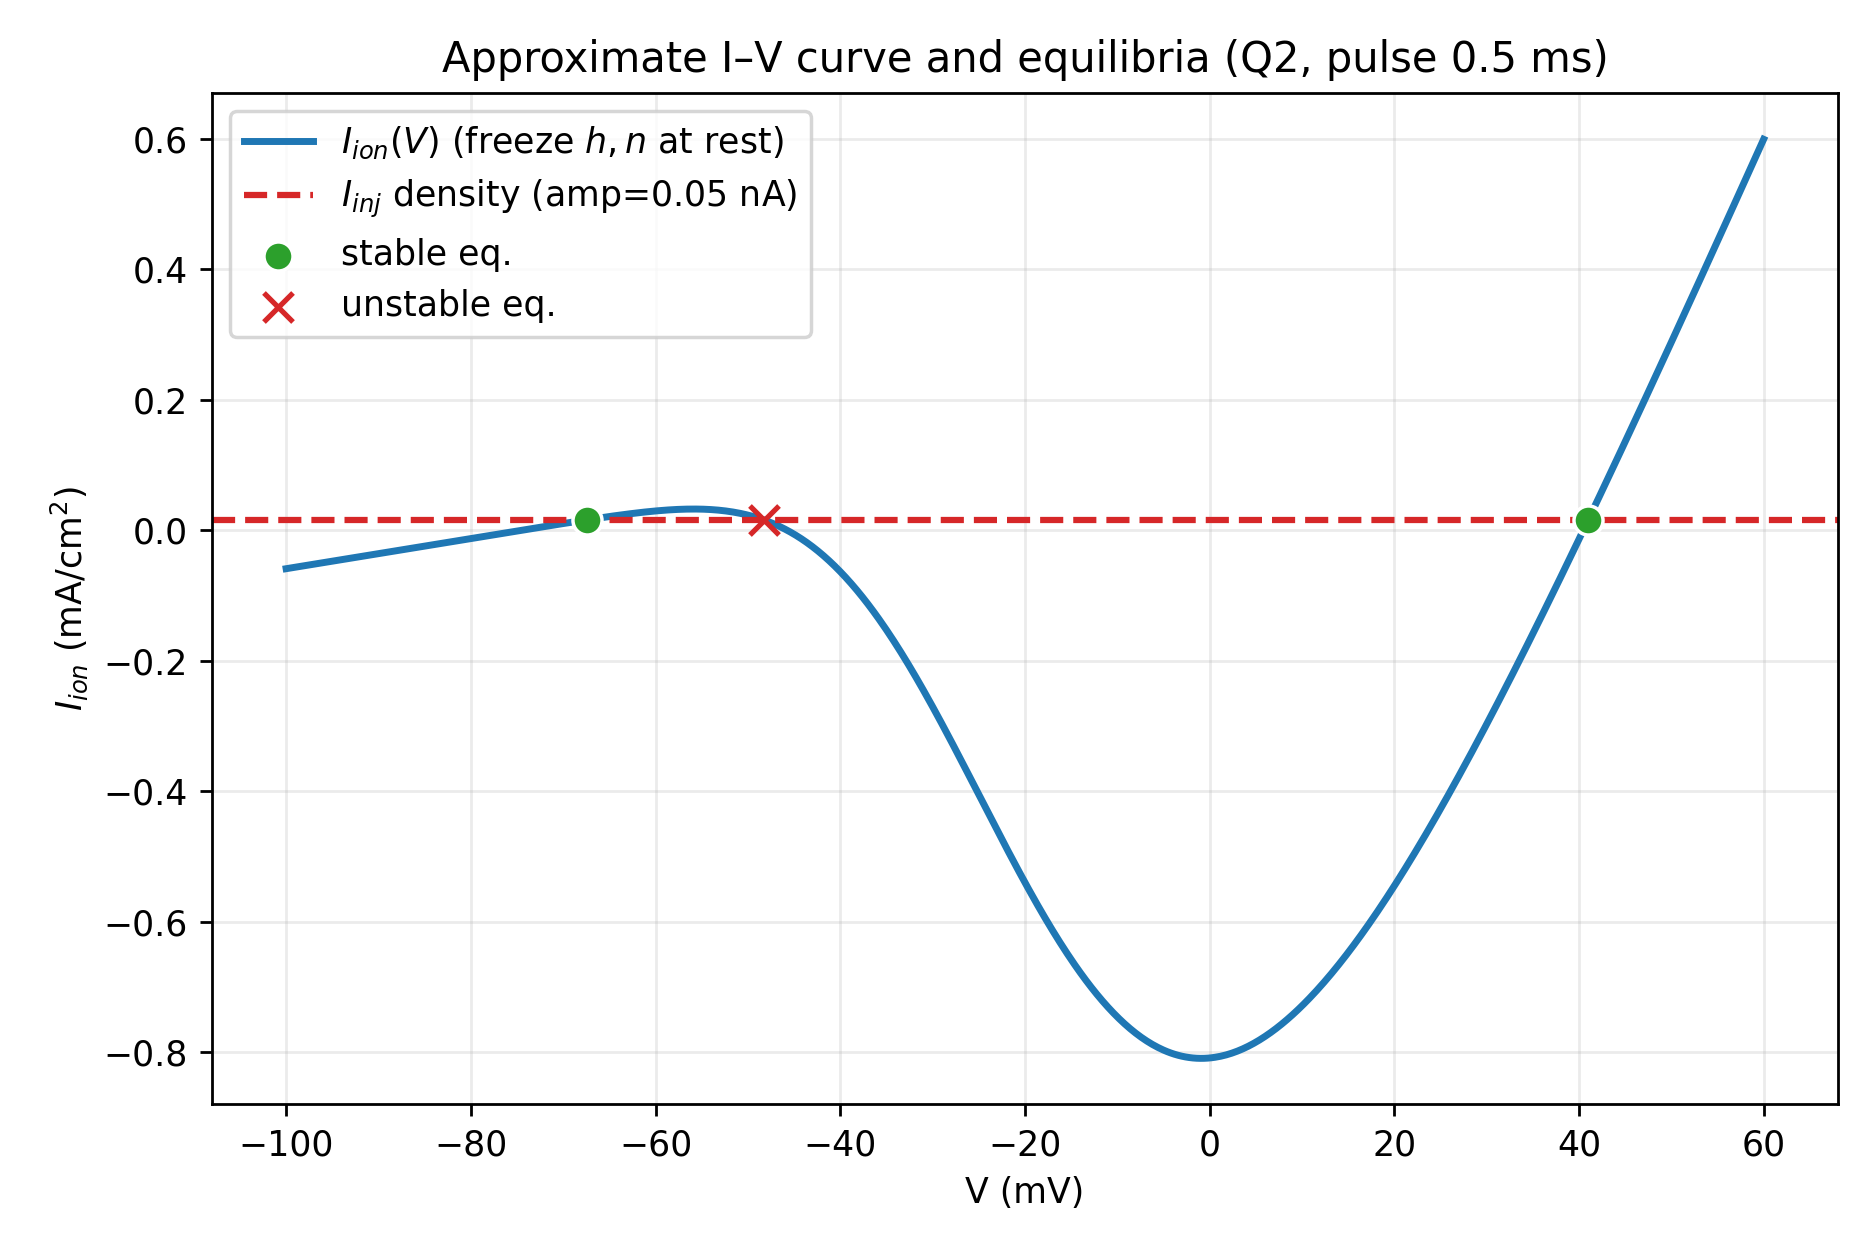
\includegraphics[width=0.80\linewidth]{Project_Code/Question_2/iv_curve_equilibria.png}
    \captionof{figure}{Approximate $I$--$V$ curve for the fast-gate analysis (example for a $0.5\,$ms pulse). Intersections with the horizontal line $I_{\mathrm{inj}}$ define equilibria; slope at the intersection determines stability (green: stable, red: unstable).}
    \label{fig:q2_iv}
\end{center}
\end{answerbox}

\clearpage

\section*{\textbf{Q3.} Revisit Hodgkin--Huxley (1952): The Dual Effect of Membrane Potential on Sodium Conductance}

In this problem, you will loosely reproduce the logic of Hodgkin and Huxley's 1952 paper
\textit{The dual effect of membrane potential on sodium conductance in the giant axon of Loligo}.\\

\noindent\textbf{Background.}
Hodgkin and Huxley studied sodium \emph{inactivation} using a two-step voltage-clamp protocol.
The membrane potential was first shifted to a \emph{conditioning voltage} $V_0$ for some duration $T_0$,
and then stepped to a fixed \emph{test voltage} $V_{\mathrm{test}}$.
They examined how the sodium current during the test step depended on the preceding conditioning step. \\

\noindent\textbf{Experiment.}
Implement a two-step voltage-clamp protocol in your model:

\begin{itemize}
    \item first hold the membrane at a conditioning voltage $V_0$ for a duration $T_0$;
    \item then step the membrane to a fixed test voltage $V_{\mathrm{test}}$ and record the sodium current.
\end{itemize}

Explore how the sodium current during the test step changes with:

\begin{enumerate}
    \item the \emph{duration} $T_0$ of the conditioning step, with $V_0$ fixed;
    \item the \emph{amplitude} of the conditioning voltage $V_0$, with $T_0$ long enough for the effect to approach steady state.
\end{enumerate}

You should choose reasonable values of $V_0$, $T_0$, and $V_{\mathrm{test}}$, and clearly explain your choices.\\

\noindent\textbf{Report requirements.}
In your report, briefly summarize the logic of this two-step protocol:
what is the role of the conditioning step, and what is the role of the test step?

Then describe your findings:

\begin{itemize}
    \item How does increasing the duration $T_0$ at a fixed $V_0$ affect the sodium current measured during the test step?
    \item How does changing the conditioning voltage $V_0$ affect the sodium current during the test step?
    \item What do these results suggest about sodium-channel inactivation and the \emph{availability} of the sodium-carrying system?
\end{itemize}

Finally, relate your observations to the Hodgkin--Huxley gating variable $h$:
explain qualitatively why a depolarized conditioning step tends to reduce the sodium current evoked by the later test step,
whereas a hyperpolarized conditioning step tends to restore it.

\textbf{Hint.}
In the original paper, the conditioning step was used to alter the degree of sodium inactivation,
while the fixed test step was used to probe how much sodium conductance could still be activated afterward. 

\textbf{Remark.}
The goal of this problem is not an exact historical reproduction of every number in the original experiments,
but to understand the experimental idea:
membrane potential has a dual effect on sodium conductance --- it helps determine both how strongly sodium channels can open and how much of the sodium system remains available for opening afterward. 

\begin{answerbox}
\textbf{Results.} Figure~\ref{fig:q3_main} shows the responses to the two-step voltage-clamp protocol. The top panels plot the Na current $I_{\mathrm{Na}}$ during the \emph{test step}; the bottom panels show the corresponding dynamics of the inactivation gate $h$ during conditioning and test.
\begin{center}
    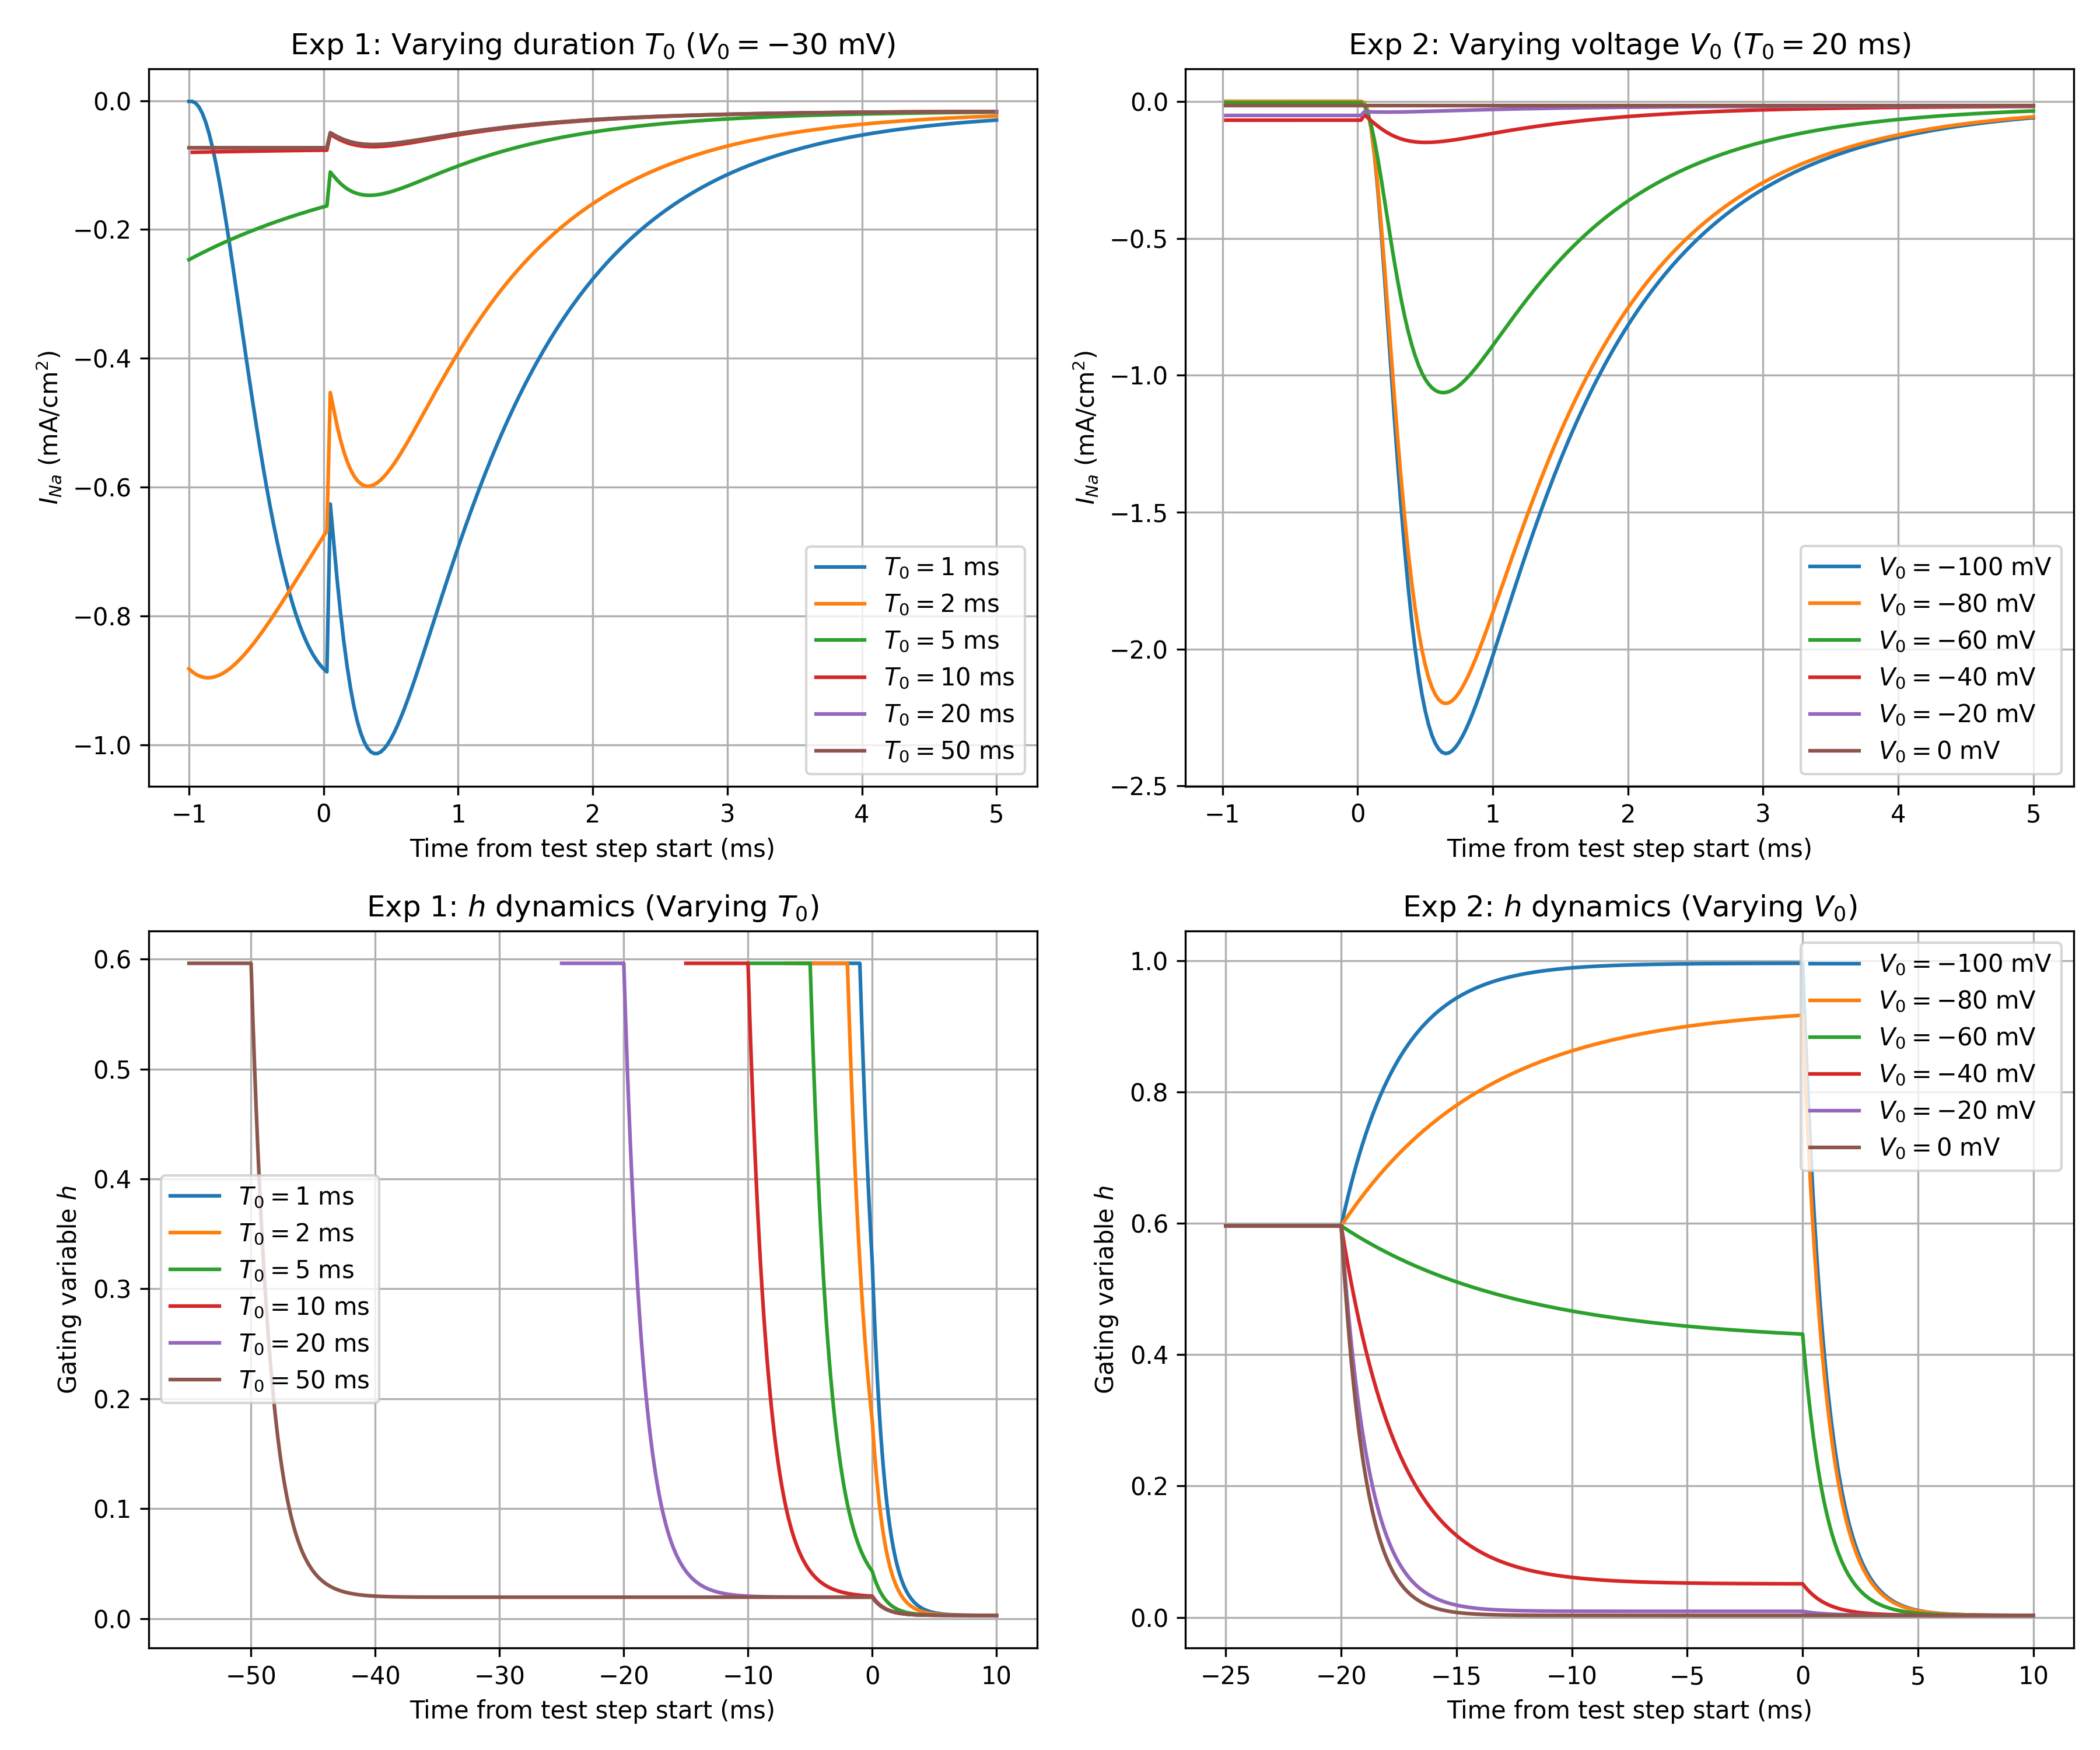
\includegraphics[width=0.98\linewidth]{Project_Code/Question_3/Figure_3.png}
    \captionof{figure}{Responses to the two-step voltage-clamp protocol. Top: test-step $I_{\mathrm{Na}}$. Bottom: $h$ dynamics during conditioning and test.}
    \label{fig:q3_main}
\end{center}

\textbf{Logic of the two-step protocol (Report requirements).}
\begin{itemize}
    \item \textbf{Conditioning step ($V_0,T_0$):} manipulates and sets the degree of Na inactivation by holding the membrane at different voltages for different durations.
    \item \textbf{Test step ($V_{\mathrm{test}}$):} uses a fixed strong depolarization to probe how many Na channels remain \emph{available} (not inactivated). The resulting peak/early $I_{\mathrm{Na}}$ reflects the availability set by conditioning.
\end{itemize}

\textbf{Parameter choices (from our implementation).}
\begin{itemize}
    \item $V_{\mathrm{test}}=0$\,mV: a strong depolarized test voltage makes activation rapid and highlights the effect of inactivation/availability.
    \item Duration experiment: fix $V_0=-30$\,mV and increase $T_0$ to observe how inactivation accumulates over time.
    \item Voltage experiment: fix $T_0=20$\,ms (long compared with $\tau_h$) so that $h$ approaches its steady-state $h_\infty(V_0)$ before the test step.
\end{itemize}

\textbf{Findings (Report requirements).}
\begin{itemize}
    \item \textbf{Effect of increasing $T_0$ (fixed depolarized $V_0$):} increasing $T_0$ causes the peak inward Na current during the test step to progressively decrease until it plateaus.
    \item \textbf{Effect of changing $V_0$ (long $T_0$):} hyperpolarized conditioning voltages (e.g., $-100$\,mV) produce very large inward Na currents in the test step, whereas sufficiently depolarized conditioning voltages (e.g., $>-40$\,mV) produce substantially smaller currents.
    \item \textbf{Implication (availability):} the conditioning step controls how much of the Na system remains available for later activation; availability depends on both voltage level and how long the membrane is held there.
    \item \textbf{Transient jump at $t=0$:} at the instant the membrane is stepped from $V_0$ to $V_{\mathrm{test}}$, $V$ changes immediately but gating variables cannot. Since $I_{\mathrm{Na}}=g_{\mathrm{Na}}(V-E_{\mathrm{Na}})$, the sudden change in driving force produces an instantaneous change in current magnitude before the subsequent activation transient.
\end{itemize}

\textbf{Relation to the HH inactivation gate $h$ (Report requirements).} Depolarized conditioning drives $h_\infty$ toward $0$ so $h$ decays and Na channels become inactivated; the later test step then evokes a much smaller peak $I_{\mathrm{Na}}$. Hyperpolarized conditioning drives $h_\infty$ toward $1$, promoting de-inactivation and restoring availability, which yields a larger test-step Na current. Because $m$ is much faster than $h$ ($\tau_m\ll\tau_h$), stepping to the same $V_{\mathrm{test}}$ makes $m$ follow nearly the same rapid trajectory across trials; thus the trial-to-trial differences are dominated by $h$ (availability).
\end{answerbox}

\clearpage

\section*{\textbf{Q4.} Neuron's responses to different protocols of current injection}

\textbf{Experiment.}
Now there are three different protocols for current injection, the neuron will immediately generate an action potential when $I_0$ is given (protocol A). 
What do you expect about the neuron’s response to protocol B and C?
(e.g. the delay of action potentials when $I_0$ is given)
\textit{Check the results with \textsc{NEURON}} and submit your plots for each protocol.

\begin{figure}[H]
    \centering
    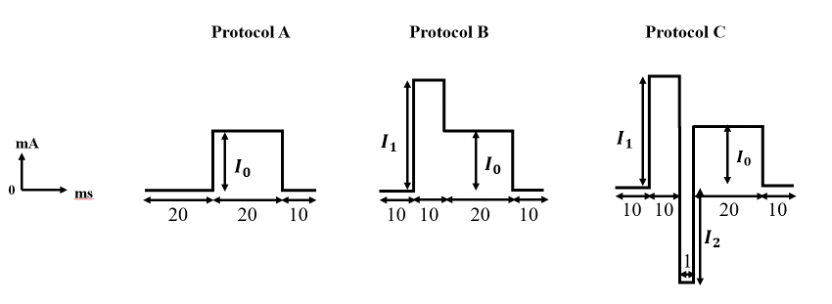
\includegraphics[width=0.8\linewidth]{figures/protocols.png}
\end{figure}

\noindent\textbf{Parameter set}:
\[I_0=\SI{0.1}{\nano\ampere},\quad I_1=\SI{1.0}{\nano\ampere},\quad I_2=\SI{-1.0}{\nano\ampere}.\]

\noindent\textbf{Report requirements.}
In your report, \textit{include all plots} and \textit{explain} your findings from the aspect of the (in)activation of ion channels.

\begin{answerbox}
\textbf{Results.} Figure~\ref{fig:q4_main} shows the voltage response and the Na inactivation variable $h$ under protocols A--C.
\begin{center}
    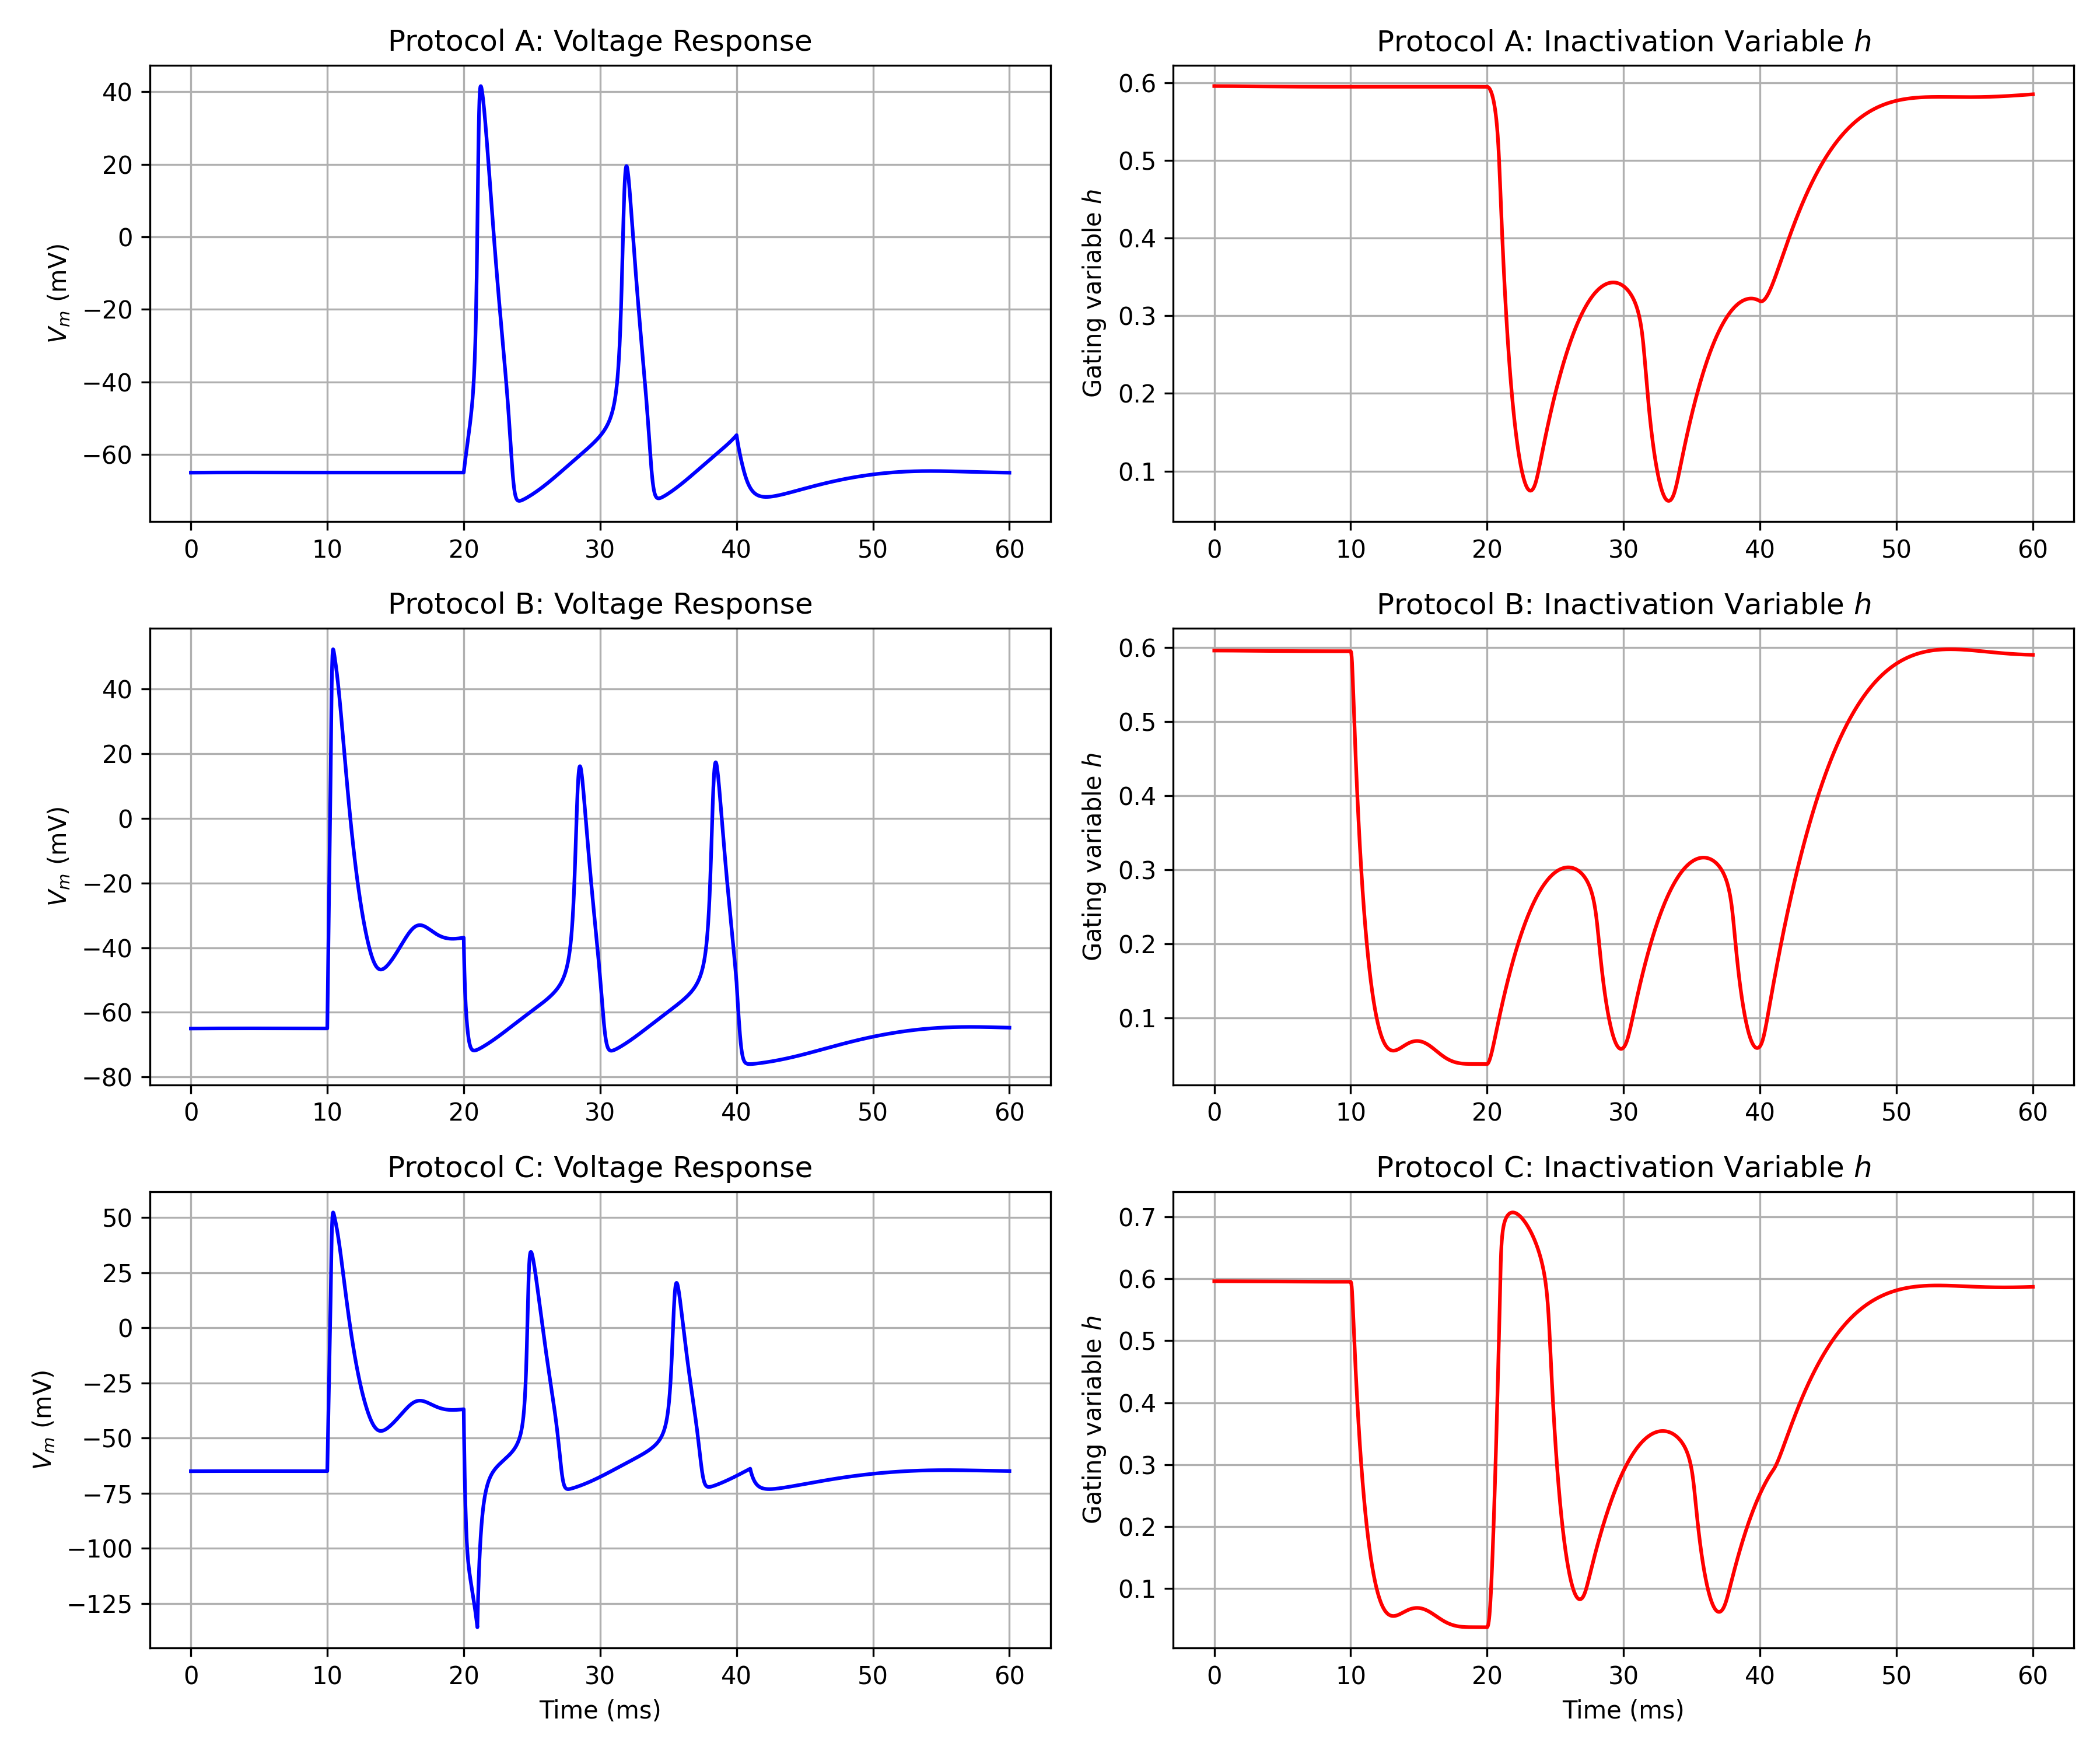
\includegraphics[width=0.98\linewidth]{Project_Code/Question_4/Figure_4.png}
    \captionof{figure}{Q4 results. Left: membrane voltage $V_m(t)$; Right: Na inactivation gate $h(t)$ under three current-injection protocols.}
    \label{fig:q4_main}
\end{center}

\textbf{Expectation (Report requirements: explain from ion-channel (in)activation).}
\begin{itemize}
    \item \textbf{Protocol A:} the neuron starts near rest with relatively high Na availability ($h\approx 0.6$), so a sustained depolarizing $I_0$ should elicit a spike with minimal delay.
    \item \textbf{Protocol B:} the strong pre-pulse $I_1$ drives spiking and deep Na inactivation ($h\to 0$). Because $I_0$ follows immediately and keeps the membrane depolarized, $h$ cannot recover quickly; thus $I_0$ is expected to fail or to trigger a spike only after a long delay.
    \item \textbf{Protocol C:} after $I_1$, the brief hyperpolarizing pulse $I_2$ rapidly increases $h$ (de-inactivation), effectively ``resetting'' excitability; therefore the delay under the subsequent $I_0$ should be reduced relative to protocol B.
\end{itemize}

\textbf{Verification with simulation (what the plot shows).} Our results match these expectations. In protocol B, $h$ remains suppressed and recovers slowly after $I_1$, so the neuron is stuck in a refractory-like state and fires only after a long delay (about $7$--$8$\,ms after $I_0$). In protocol C, the strong negative pulse produces a rapid upward jump in $h$, and the neuron fires sooner (about $4$--$5$\,ms after $I_0$).
\end{answerbox}

\clearpage

\section*{\textbf{Q5.} Calcium Channels}

Until now we have only considered 2 types of ion channels ($\mathrm{Na}^+,\,\mathrm{K}^+$), however, voltage-gated calcium channels are also activated when neurons fire action potentials. 
Experiments show that slow calcium spikes provide the driving force for a long burst of rapidly emitted sodium spikes. 
\textit{T-type calcium channels} are low-voltage-activated calcium channels found in the cardiac muscle cells and thalamus nerve cells. \\

\noindent\textbf{Experiment.}
Add CaT channels to the HH model in \textbf{Q1}. Plot the voltage response of your model (like how the response differs from the original HH model's).\\

\noindent\textbf{Parameter set}:
\[\texttt{hh1.el}=\SI{-65}{\milli\volt}.\]
(Maybe you can explain why soma will spontaneously spike when $\texttt{hh1.el}=\SI{-54.3}{\milli\volt}$, if you have extra time.)\\

\noindent\textbf{Report requirements.}
In your report, \textit{include all plots} and \textit{interpret} your finding from the aspect of the (in)activation of ion channels.

\begin{answerbox}
\textbf{Results.}
\begin{center}
    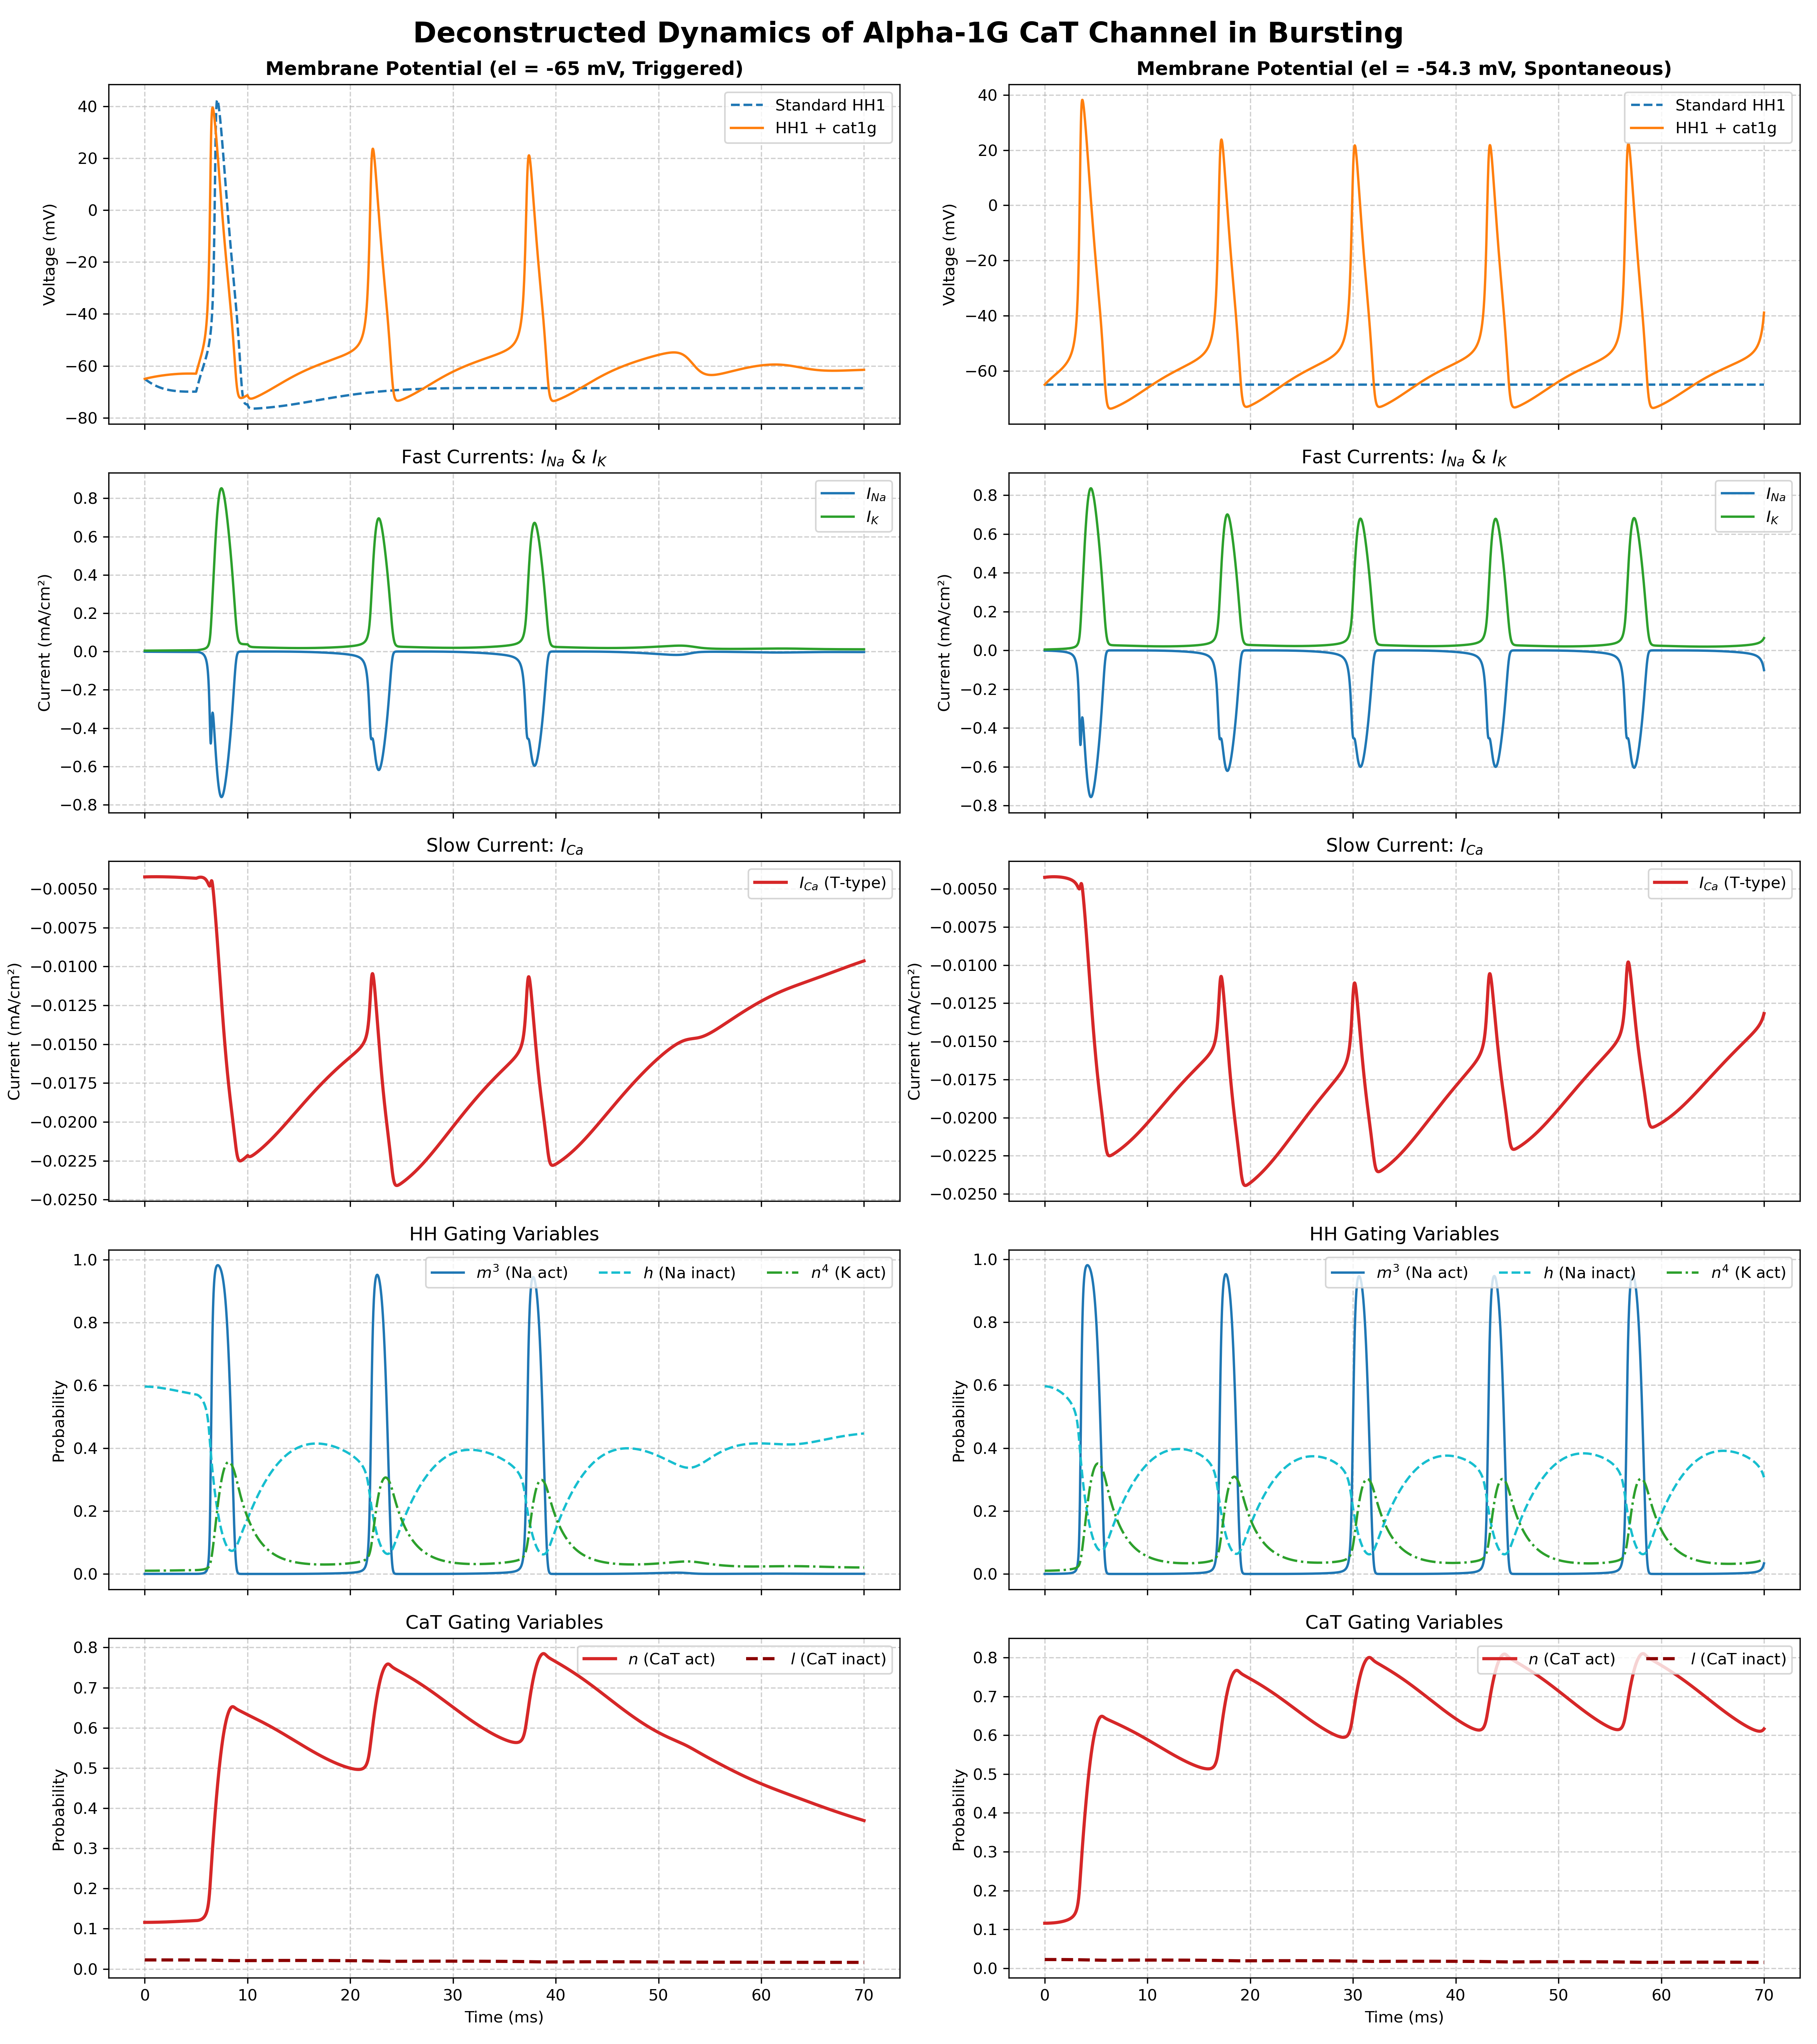
\includegraphics[width=1.0\textwidth]{Project_Code/Question_5/Q5_Separated_Dynamics.png}
    \captionof{figure}{Deconstructed dynamics of Alpha-1G T-type Calcium Channels (\texttt{cat1g}) during neuronal firing. The left column shows the triggered response at a resting potential of $-65 \text{ mV}$ (with a $5 \text{ ms}$ pulse), and the right column shows spontaneous firing at $-54.3 \text{ mV}$ (no pulse). Rows display: (1) Membrane Potential, (2) Fast HH Currents ($I_{Na}$, $I_{K}$), (3) Slow CaT Current ($I_{Ca}$), (4) HH Gating Variables ($m^3, h, n^4$), and (5) CaT Gating Variables ($n, l$).}
    \label{fig:q5_calcium}
\end{center}

\textbf{1. Overview of the Experiment}
\begin{itemize}
    \item We introduced T-type (low-voltage-activated) calcium channels (\texttt{cat1g}) into the standard Hodgkin-Huxley (HH) model.
    \item To fully understand the underlying mechanics, we explicitly decoupled and plotted the fast ion currents ($I_{Na}$, $I_{K}$), the slow calcium current ($I_{Ca}$), and the gating variables for both channel types.
    \item Two experimental conditions were tested:
    \begin{itemize}
        \item \textbf{Left Column ($E_L = -65 \text{ mV}$):} Standard resting potential with a brief $5 \text{ ms}$ depolarizing pulse ($0.05 \text{ nA}$) to trigger firing.
        \item \textbf{Right Column ($E_L = -54.3 \text{ mV}$):} Elevated resting potential with no external stimulus, demonstrating spontaneous bursting behavior.
    \end{itemize}
\end{itemize}

\textbf{2. Voltage Response Analysis}
\begin{itemize}
    \item \textbf{Standard HH Model (dashed blue):} At $E_L = -65 \text{ mV}$, the original HH model produces only a single action potential in response to the stimulus, quickly returning to rest. At $E_L = -54.3 \text{ mV}$, it remains at a stable depolarized plateau without firing.
    \item \textbf{HH + CaT Model (solid orange):} The addition of T-type calcium channels fundamentally transforms the firing pattern:
    \begin{itemize}
        \item At $E_L = -65 \text{ mV}$: Instead of a single spike, the neuron exhibits a \textit{burst of three action potentials}. The initial spike is triggered by the external pulse, but subsequent spikes are generated endogenously through the slow calcium current dynamics.
        \item At $E_L = -54.3 \text{ mV}$: The neuron displays \textit{rhythmic spontaneous bursting} with approximately 5 spikes over 70 ms, without any external stimulation.
    \end{itemize}
\end{itemize}

\textbf{3. Ion Channel Activation Dynamics: The Mechanism of Bursting}

The bursting behavior arises from the interaction between fast sodium/potassium currents and the slow T-type calcium current, operating on distinct timescales:
\begin{itemize}
    \item \textbf{Fast Currents ($I_{Na}$ and $I_{K}$):} The sodium and potassium currents exhibit rapid, transient activation during each action potential. $I_{Na}$ peaks sharply at spike onset, followed immediately by $I_{K}$ which drives repolarization. These currents are nearly identical in both conditions.
    \item \textbf{Slow Calcium Current ($I_{Ca}$):} The T-type calcium current is critical:
    \begin{itemize}
        \item \textit{Low-threshold:} Activated at relatively depolarized potentials (near $-60 \text{ mV}$).
        \item \textit{Slow kinetics:} Evolves over tens of milliseconds.
        \item \textit{Depolarizing:} The inward calcium current provides a slow depolarizing drive that gradually brings the membrane potential back toward threshold after each spike.
    \end{itemize}
\end{itemize}

\textbf{4. Gating Variable Analysis}
\begin{itemize}
    \item \textbf{HH Gating Variables:} The activation ($m^3$, $n^4$) and inactivation ($h$) variables show classic HH dynamics. Notably, the sodium inactivation variable $h$ accumulates partial inactivation during rapid firing, contributing to spike frequency adaptation within bursts.
    \item \textbf{CaT Gating Variables:} The T-type calcium channel has two distinct gates:
    \begin{itemize}
        \item \textbf{Activation gate ($n$):} Shows slow, cumulative activation between spikes, reaching peak values of $\sim 0.8$.
        \item \textbf{Inactivation gate ($l$):} Remains near zero throughout the simulation, indicating that the T-type channels do not fully inactivate, allowing continuous depolarizing drive.
    \end{itemize}
\end{itemize}

\textbf{5. Why $E_L = -54.3 \text{ mV}$ Causes Spontaneous Firing}
\begin{itemize}
    \item \textbf{Proximity to Threshold:} At $-54.3 \text{ mV}$, the resting potential partially activates the T-type calcium channels.
    \item \textbf{Slow Depolarizing Ramp:} The persistent calcium influx ($I_{Ca}$) creates a gradual depolarizing current that slowly charges the membrane capacitance.
    \item \textbf{Regenerative Feedback:} Once reaching sodium threshold, a fast spike is triggered. The subsequent repolarization is not sufficient to fully deactivate the calcium channels, allowing the cycle to restart.
    \item \textbf{Limit Cycle:} The system transitions from a stable fixed point to a stable periodic orbit due to the interaction of fast HH currents and slow calcium currents.
\end{itemize}

\vspace{1em}
\begin{center}
    \captionof{table}{Summary of firing patterns and underlying mechanisms}
    \label{tab:q5_summary}
    \begin{tabular}{@{}p{3.5cm}p{3cm}p{4cm}p{3cm}@{}}
    \toprule
    \textbf{Condition} & \textbf{Firing Pattern} & \textbf{Mechanism} & \textbf{Role of $I_{Ca}$} \\
    \midrule
    HH only, $E_L = -65\,$mV & Single spike & External stimulus only & N/A \\
    HH + CaT, $E_L = -65\,$mV & Burst of 3 spikes & External trigger + calcium rebound & Interspike depolarization \\
    HH only, $E_L = -54.3\,$mV & No firing & Stable depolarization & N/A \\
    HH + CaT, $E_L = -54.3\,$mV & Rhythmic bursting & Endogenous pacemaker & Driver of oscillation \\
    \bottomrule
    \end{tabular}
\end{center}
\end{answerbox}

\clearpage

\section*{\textbf{Q6.} Fast Spiking}

\noindent\textbf{Experiment.}
Inject a stronger current ($I=\SI{0.5}{\nano\ampere}$) into the point neuron. 
Does the neuron generate a sustained train of action potentials?
\textit{Plot} the voltage response.
\textit{Explain} why the neuron does or does not continue firing.

Then try to make the model generate faster spikes (i.e.\ shorter interspike intervals) by \textit{modifying the parameters} in \texttt{hh1.mod}.

For \textbf{Part 2}, submit all plots and codes.\\

\noindent\textbf{Report requirements.}
In your report, \textit{describe and explain} what happens when a stronger current is injected.
Then \textit{present} your modified parameter set and \textit{explain} why the new model exhibits fast-spiking behavior.
Remember to \textit{include all plots}.

\begin{answerbox}
\textbf{Results.} 
\begin{center}
    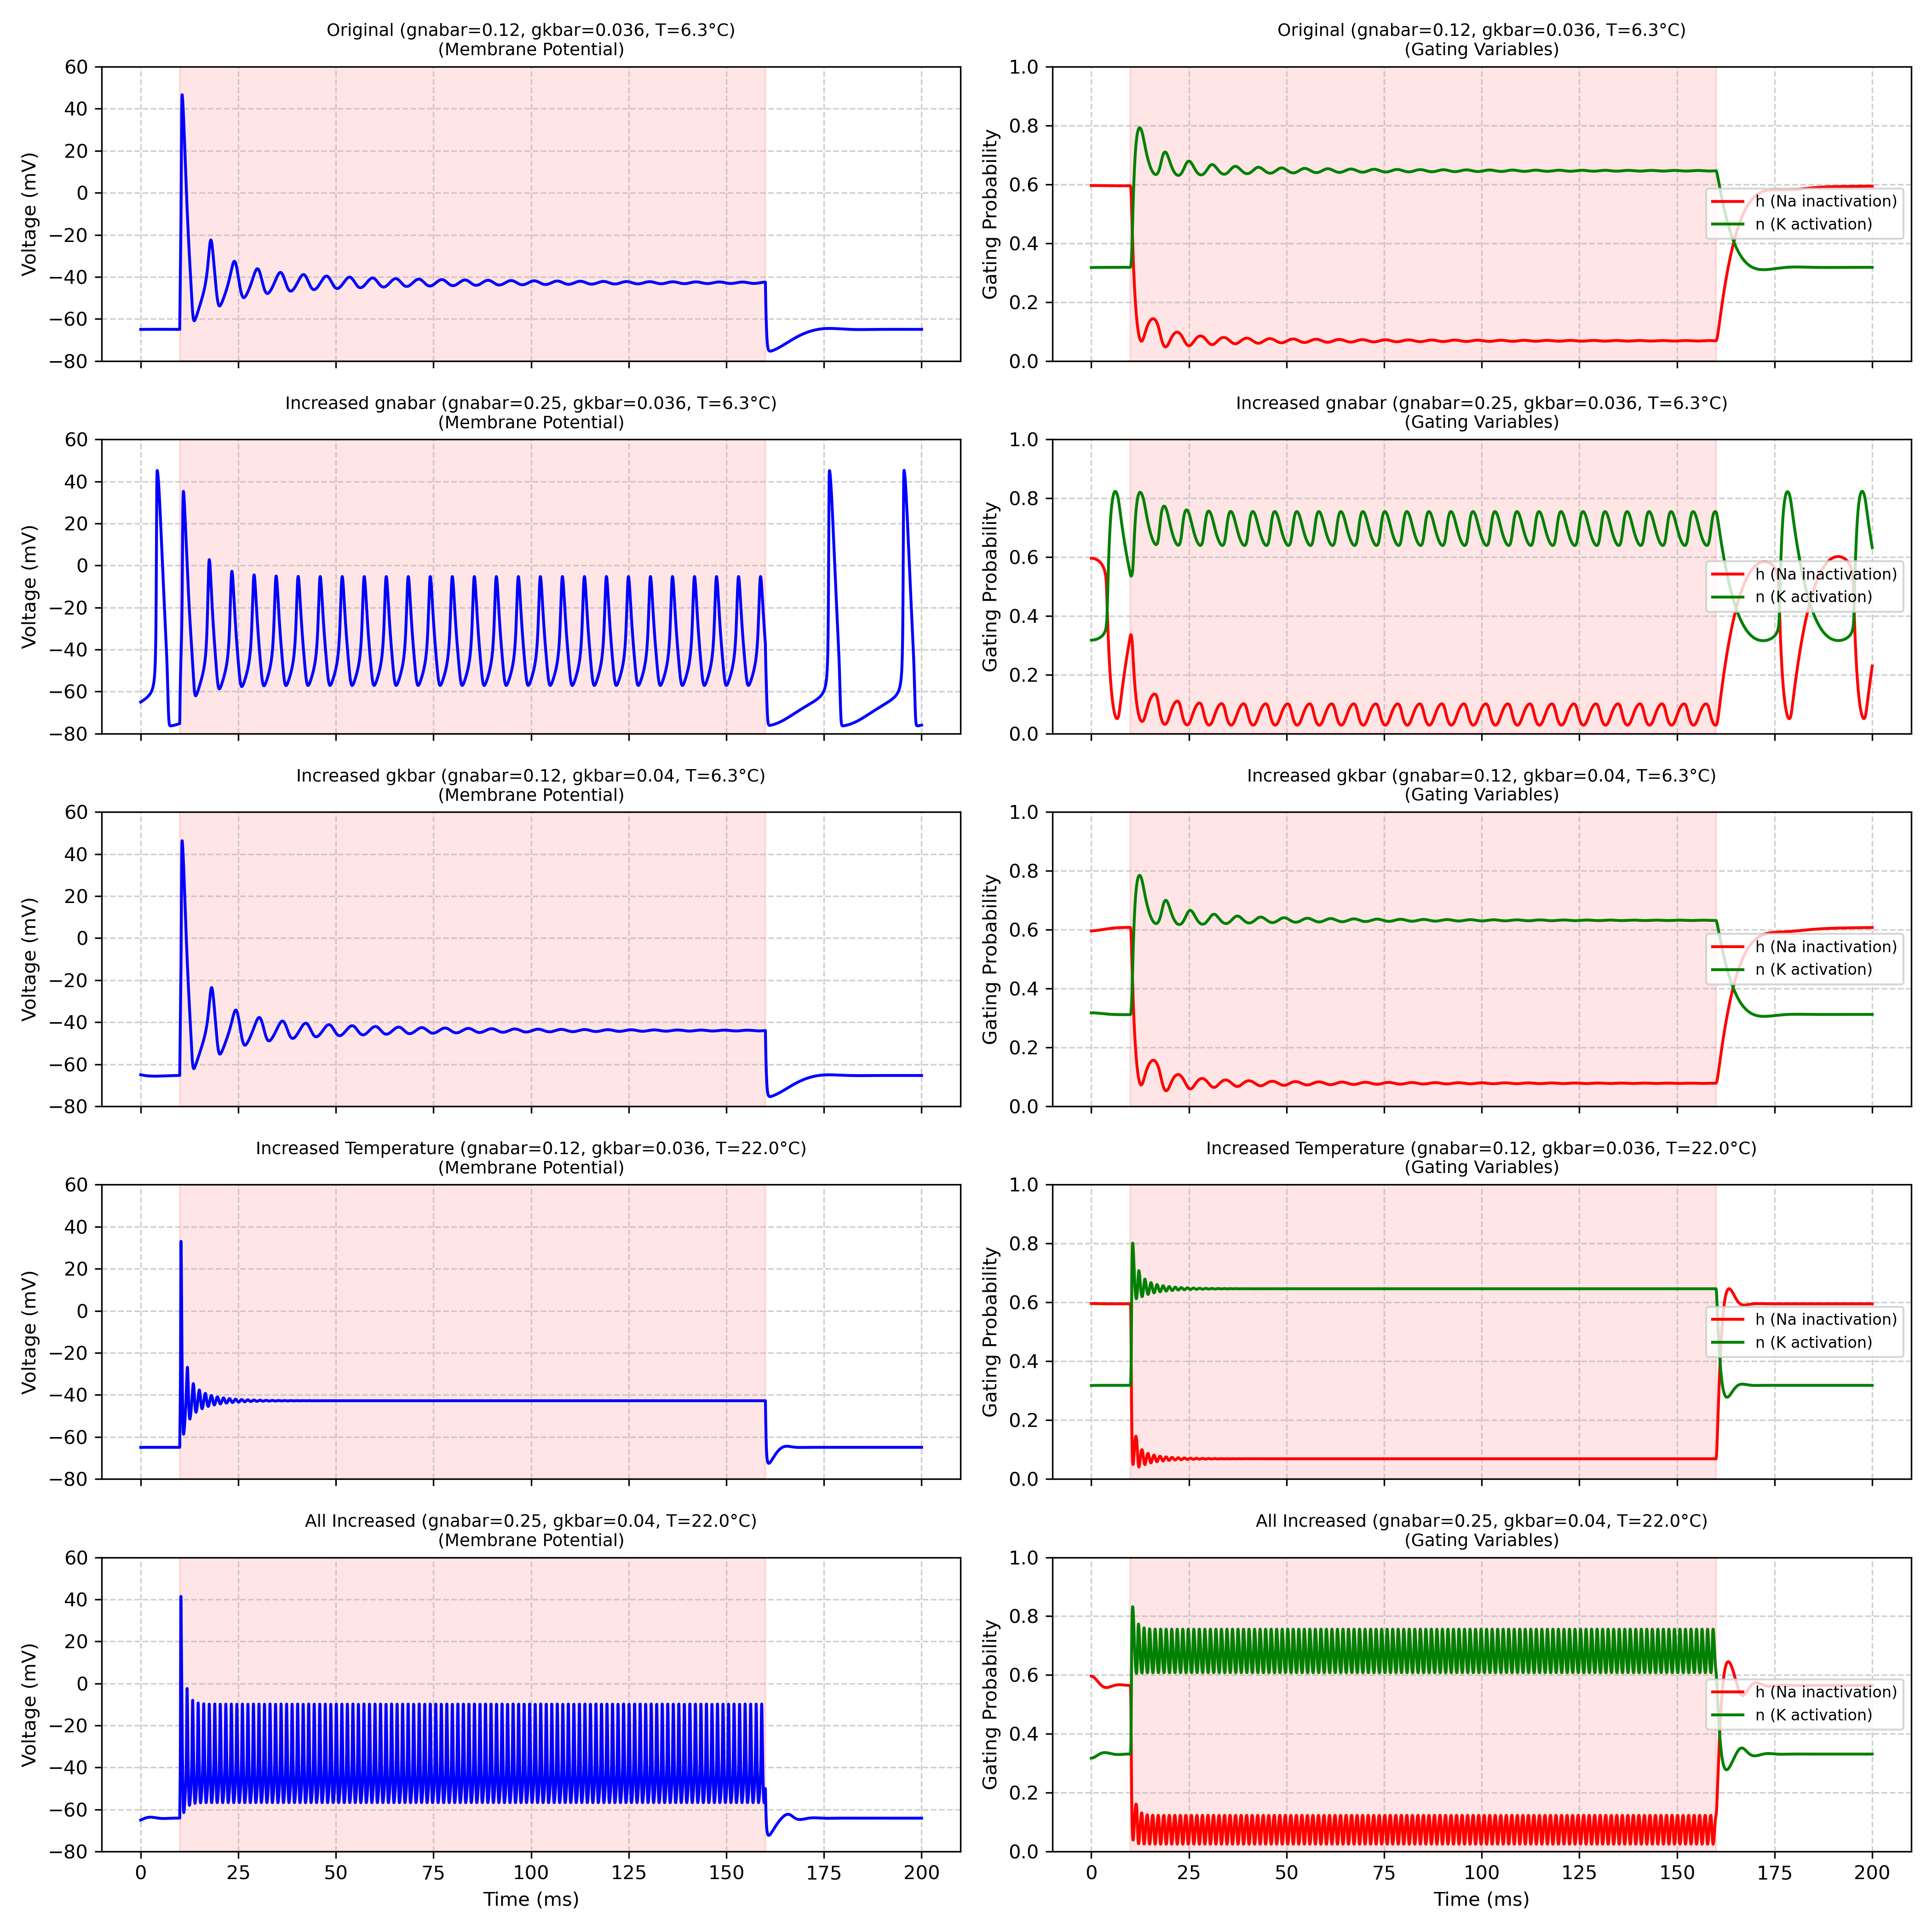
\includegraphics[width=1.0\textwidth]{Project_Code/Question_5/Controlled_Variable_Comparison.png}
    \captionof{figure}{Responses of the HH neuron under $I = 0.5\ \text{nA}$ stimulus. The left column shows membrane voltage, and the right column shows the gating variables $h$ (red) and $n$ (green). The red shaded region indicates the stimulus duration.}
    \label{fig:q6_controlled}
\end{center}

\textbf{1. Overview of the Experiment}
\begin{itemize}
    \item We injected a strong, sustained current ($0.5\ \text{nA}$) into a single-compartment Hodgkin-Huxley neuron model.
    \item We evaluated whether the neuron could sustain continuous action potentials under this extreme drive, analyzing both voltage responses and gating variable dynamics.
    \item We then conducted a controlled variable simulation to find an optimal parameter set ($\bar{g}_{Na}$, $\bar{g}_K$, and Temperature) that overcomes response failure and forces the model to produce fast spikes.
\end{itemize}

\textbf{2. Voltage Response Analysis}
\begin{itemize}
    \item \textbf{Original Model ($6.3^\circ\text{C}$):} As shown in the top row of Figure \ref{fig:q6_controlled}, the neuron generates only a single initial spike followed by a steady depolarized plateau. It fails to sustain continuous firing.
    \item \textbf{Modified Model ($22.0^\circ\text{C}$):} As shown in the bottom row of Figure \ref{fig:q6_controlled}, the optimized model overcomes the plateau and successfully exhibits a sustained, continuous train of high-frequency spikes.
\end{itemize}

\textbf{3. Ion Channel Dynamics: The Mechanism of Depolarization Block}

The failure to sustain firing in the original model is due to a phenomenon known as \textbf{depolarization block}. By analyzing the variables, we observe:
\begin{itemize}
    \item \textbf{Extreme Depolarization:} The excessive $0.5\ \text{nA}$ current rapidly drives the membrane potential to a highly depolarized state ($\sim -40\ \text{mV}$).
    \item \textbf{Sodium Channel Inactivation:} At this sustained high voltage, the sodium inactivation variable $h$ rapidly drops to near 0. 
    \item \textbf{Failure to Repolarize:} Because the outward potassium current ($\bar{g}_K = 0.036$) is insufficient to overcome the massive injected inward current, the membrane cannot repolarize to negative resting potentials. Consequently, the $h$ gate cannot de-inactivate (recover), locking the sodium channels in a closed/inactivated state.
\end{itemize}

\textbf{4. Modifying Parameters for Fast Spiking}
\begin{itemize}
    \item To overcome the depolarization block, we tested multiple parameter configurations (summarized in Table \ref{tab:param_alt_q6} below).
    \item \textbf{Optimal Parameter Set:} The optimal modifications to allow sustained, extremely fast spiking are: \textbf{$\bar{g}_{Na} = 0.25$, $\bar{g}_K = 0.04$, and Temperature $= 22.0^\circ\text{C}$}.
    \item \textit{Note:} Elevating the temperature via \texttt{h.celsius} universally accelerates the $\alpha$ and $\beta$ rate constants in the \texttt{hh1.mod} file via the $Q_{10}$ scaling factor, effectively shortening the kinetic time constants.
\end{itemize}

\textbf{5. Why the New Model Exhibits Fast Spiking}

The combined modifications prevent the gating variables from getting ``stuck'' at steady-state values, unlocking a high-frequency limit cycle:
\begin{itemize}
    \item \textbf{Accelerated Kinetics (High Temp):} The elevated temperature ($22^\circ\text{C}$) dramatically speeds up the channel gating dynamics. The $h$ and $n$ variables oscillate at a much higher frequency, allowing the $h$ gate to recover from inactivation in a fraction of a millisecond.
    \item \textbf{Enhanced Depolarizing Drive (High $\bar{g}_{Na}$):} Increasing sodium conductance to $0.25\ \text{S/cm}^2$ ensures that once the $h$ gate slightly recovers, the influx of $Na^+$ is powerful enough to instantly trigger the next spike, fighting against the strong injected current.
    \item \textbf{Slightly Increased Repolarization (High $\bar{g}_K$):} Nudging potassium conductance to $0.04$ assists in bringing the voltage down just enough during the rapid refractory period to allow the accelerated $h$ gate to reset.
\end{itemize}

\vspace{1em}
\begin{center}
    \captionof{table}{Parameter configurations and resulting firing patterns under $I = 0.5\ \text{nA}$}
    \label{tab:param_alt_q6}
    \begin{tabular}{@{}p{3.5cm}cccp{6cm}@{}}
    \toprule
    \textbf{Condition} & $\bar{g}_{Na}$ & $\bar{g}_K$ & $T$ ($^\circ\text{C}$) & \textbf{Observed Behavior} \\
    \midrule
    Original & 0.12 & 0.036 & 6.3 & Depolarization block (single spike, $h \approx 0$). \\
    Increased $\bar{g}_{Na}$ & 0.25 & 0.036 & 6.3 & Spiking, but exhibits adaptation and slowing down. \\
    Increased $\bar{g}_K$ & 0.12 & 0.04 & 6.3 & Depolarization block (single spike). \\
    Increased Temp. & 0.12 & 0.036 & 22.0 & Transient fast spikes rapidly decaying into a block. \\
    \textbf{All Increased} & \textbf{0.25} & \textbf{0.04} & \textbf{22.0} & \textbf{Sustained, continuous fast spiking without block.} \\
    \bottomrule
    \end{tabular}
\end{center}
\end{answerbox}


\end{document}